% Options for packages loaded elsewhere
\PassOptionsToPackage{unicode}{hyperref}
\PassOptionsToPackage{hyphens}{url}
%
\documentclass[
  8pt,
  ignorenonframetext,
]{beamer}
\usepackage{pgfpages}
\setbeamertemplate{caption}[numbered]
\setbeamertemplate{caption label separator}{: }
\setbeamercolor{caption name}{fg=normal text.fg}
\beamertemplatenavigationsymbolsempty
% Prevent slide breaks in the middle of a paragraph
\widowpenalties 1 10000
\raggedbottom
\setbeamertemplate{part page}{
  \centering
  \begin{beamercolorbox}[sep=16pt,center]{part title}
    \usebeamerfont{part title}\insertpart\par
  \end{beamercolorbox}
}
\setbeamertemplate{section page}{
  \centering
  \begin{beamercolorbox}[sep=12pt,center]{part title}
    \usebeamerfont{section title}\insertsection\par
  \end{beamercolorbox}
}
\setbeamertemplate{subsection page}{
  \centering
  \begin{beamercolorbox}[sep=8pt,center]{part title}
    \usebeamerfont{subsection title}\insertsubsection\par
  \end{beamercolorbox}
}
\AtBeginPart{
  \frame{\partpage}
}
\AtBeginSection{
  \ifbibliography
  \else
    \frame{\sectionpage}
  \fi
}
\AtBeginSubsection{
  \frame{\subsectionpage}
}
\usepackage{amsmath,amssymb}
\usepackage{lmodern}
\usepackage{iftex}
\ifPDFTeX
  \usepackage[T1]{fontenc}
  \usepackage[utf8]{inputenc}
  \usepackage{textcomp} % provide euro and other symbols
\else % if luatex or xetex
  \usepackage{unicode-math}
  \defaultfontfeatures{Scale=MatchLowercase}
  \defaultfontfeatures[\rmfamily]{Ligatures=TeX,Scale=1}
\fi
% Use upquote if available, for straight quotes in verbatim environments
\IfFileExists{upquote.sty}{\usepackage{upquote}}{}
\IfFileExists{microtype.sty}{% use microtype if available
  \usepackage[]{microtype}
  \UseMicrotypeSet[protrusion]{basicmath} % disable protrusion for tt fonts
}{}
\makeatletter
\@ifundefined{KOMAClassName}{% if non-KOMA class
  \IfFileExists{parskip.sty}{%
    \usepackage{parskip}
  }{% else
    \setlength{\parindent}{0pt}
    \setlength{\parskip}{6pt plus 2pt minus 1pt}}
}{% if KOMA class
  \KOMAoptions{parskip=half}}
\makeatother
\usepackage{xcolor}
\newif\ifbibliography
\usepackage{color}
\usepackage{fancyvrb}
\newcommand{\VerbBar}{|}
\newcommand{\VERB}{\Verb[commandchars=\\\{\}]}
\DefineVerbatimEnvironment{Highlighting}{Verbatim}{commandchars=\\\{\}}
% Add ',fontsize=\small' for more characters per line
\usepackage{framed}
\definecolor{shadecolor}{RGB}{248,248,248}
\newenvironment{Shaded}{\begin{snugshade}}{\end{snugshade}}
\newcommand{\AlertTok}[1]{\textcolor[rgb]{0.94,0.16,0.16}{#1}}
\newcommand{\AnnotationTok}[1]{\textcolor[rgb]{0.56,0.35,0.01}{\textbf{\textit{#1}}}}
\newcommand{\AttributeTok}[1]{\textcolor[rgb]{0.77,0.63,0.00}{#1}}
\newcommand{\BaseNTok}[1]{\textcolor[rgb]{0.00,0.00,0.81}{#1}}
\newcommand{\BuiltInTok}[1]{#1}
\newcommand{\CharTok}[1]{\textcolor[rgb]{0.31,0.60,0.02}{#1}}
\newcommand{\CommentTok}[1]{\textcolor[rgb]{0.56,0.35,0.01}{\textit{#1}}}
\newcommand{\CommentVarTok}[1]{\textcolor[rgb]{0.56,0.35,0.01}{\textbf{\textit{#1}}}}
\newcommand{\ConstantTok}[1]{\textcolor[rgb]{0.00,0.00,0.00}{#1}}
\newcommand{\ControlFlowTok}[1]{\textcolor[rgb]{0.13,0.29,0.53}{\textbf{#1}}}
\newcommand{\DataTypeTok}[1]{\textcolor[rgb]{0.13,0.29,0.53}{#1}}
\newcommand{\DecValTok}[1]{\textcolor[rgb]{0.00,0.00,0.81}{#1}}
\newcommand{\DocumentationTok}[1]{\textcolor[rgb]{0.56,0.35,0.01}{\textbf{\textit{#1}}}}
\newcommand{\ErrorTok}[1]{\textcolor[rgb]{0.64,0.00,0.00}{\textbf{#1}}}
\newcommand{\ExtensionTok}[1]{#1}
\newcommand{\FloatTok}[1]{\textcolor[rgb]{0.00,0.00,0.81}{#1}}
\newcommand{\FunctionTok}[1]{\textcolor[rgb]{0.00,0.00,0.00}{#1}}
\newcommand{\ImportTok}[1]{#1}
\newcommand{\InformationTok}[1]{\textcolor[rgb]{0.56,0.35,0.01}{\textbf{\textit{#1}}}}
\newcommand{\KeywordTok}[1]{\textcolor[rgb]{0.13,0.29,0.53}{\textbf{#1}}}
\newcommand{\NormalTok}[1]{#1}
\newcommand{\OperatorTok}[1]{\textcolor[rgb]{0.81,0.36,0.00}{\textbf{#1}}}
\newcommand{\OtherTok}[1]{\textcolor[rgb]{0.56,0.35,0.01}{#1}}
\newcommand{\PreprocessorTok}[1]{\textcolor[rgb]{0.56,0.35,0.01}{\textit{#1}}}
\newcommand{\RegionMarkerTok}[1]{#1}
\newcommand{\SpecialCharTok}[1]{\textcolor[rgb]{0.00,0.00,0.00}{#1}}
\newcommand{\SpecialStringTok}[1]{\textcolor[rgb]{0.31,0.60,0.02}{#1}}
\newcommand{\StringTok}[1]{\textcolor[rgb]{0.31,0.60,0.02}{#1}}
\newcommand{\VariableTok}[1]{\textcolor[rgb]{0.00,0.00,0.00}{#1}}
\newcommand{\VerbatimStringTok}[1]{\textcolor[rgb]{0.31,0.60,0.02}{#1}}
\newcommand{\WarningTok}[1]{\textcolor[rgb]{0.56,0.35,0.01}{\textbf{\textit{#1}}}}
\setlength{\emergencystretch}{3em} % prevent overfull lines
\providecommand{\tightlist}{%
  \setlength{\itemsep}{0pt}\setlength{\parskip}{0pt}}
\setcounter{secnumdepth}{-\maxdimen} % remove section numbering
\newlength{\cslhangindent}
\setlength{\cslhangindent}{1.5em}
\newlength{\csllabelwidth}
\setlength{\csllabelwidth}{3em}
\newlength{\cslentryspacingunit} % times entry-spacing
\setlength{\cslentryspacingunit}{\parskip}
\newenvironment{CSLReferences}[2] % #1 hanging-ident, #2 entry spacing
 {% don't indent paragraphs
  \setlength{\parindent}{0pt}
  % turn on hanging indent if param 1 is 1
  \ifodd #1
  \let\oldpar\par
  \def\par{\hangindent=\cslhangindent\oldpar}
  \fi
  % set entry spacing
  \setlength{\parskip}{#2\cslentryspacingunit}
 }%
 {}
\usepackage{calc}
\newcommand{\CSLBlock}[1]{#1\hfill\break}
\newcommand{\CSLLeftMargin}[1]{\parbox[t]{\csllabelwidth}{#1}}
\newcommand{\CSLRightInline}[1]{\parbox[t]{\linewidth - \csllabelwidth}{#1}\break}
\newcommand{\CSLIndent}[1]{\hspace{\cslhangindent}#1}
% type setting
% ------------------------------------------------------------------------------
\usepackage[german]{babel}     

% fonts
% ------------------------------------------------------------------------------
\usefonttheme{professionalfonts}

% slide title and horizontal line
% ------------------------------------------------------------------------------
\setbeamertemplate{frametitle}{%
    \vskip-30pt \color{black}\large%
    \begin{minipage}[b][23pt]{120mm}%
    \flushleft\insertframetitle%
    \end{minipage}%
}

\setbeamertemplate{headline}										
{
\vskip10pt\hfill\hspace{3.5mm} 										 
\vskip15pt\color{black}\rule{\textwidth}{0.4pt} 					 
}

% slide number
% ---------------------------------------------------------------
\setbeamertemplate{navigation symbols}{}
\setbeamertemplate{footline}
{
\vskip5pt
\vskip2pt
\makebox[123mm]{\hspace{7.5mm}
\hfill Multivariate Datenanalyse $\vert$ 
\copyright $ $ 2023 Dirk Ostwald CC BY-SA 4.0 $\vert$ 
Folie \insertframenumber}
\vskip4pt
}

% block color scheme
% ------------------------------------------------------------------------------
% colors
\definecolor{white}{RGB}{255,255,255}
\definecolor{grey}{RGB}{235,235,235}
\definecolor{lightgrey}{RGB}{245,245,245}
\definecolor{LightBlue}{RGB}{220,220,255}
\definecolor{darkblue}{RGB}{51, 51, 153}

% definitions and theorems
\setbeamercolor{block title}{fg = black, bg = grey}
\setbeamercolor{block body}{fg = black, bg = lightgrey}

% general line spacing 
% ------------------------------------------------------------------------------
\linespread{1.3}

% local line spacing
% ------------------------------------------------------------------------------
\usepackage{setspace}

% colors
% -----------------------------------------------------------------------------
\usepackage{color}

% justified text
% ------------------------------------------------------------------------------
\usepackage{ragged2e}
\usepackage{etoolbox}
\apptocmd{\frame}{}{\justifying}{}

% bullet point lists
% -----------------------------------------------------------------------------
\setbeamertemplate{itemize item}[circle]
\setbeamertemplate{itemize subitem}[circle]
\setbeamertemplate{itemize subsubitem}[circle]
\setbeamercolor{itemize item}{fg = black}
\setbeamercolor{itemize subitem}{fg = black}
\setbeamercolor{itemize subsubitem}{fg = black}
\setbeamercolor{enumerate item}{fg = black}
\setbeamercolor{enumerate subitem}{fg = black}
\setbeamercolor{enumerate subsubitem}{fg = black}
\setbeamerfont{itemize/enumerate body}{}
\setbeamerfont{itemize/enumerate subbody}{size = \normalsize}
\setbeamerfont{itemize/enumerate subsubbody}{size = \normalsize}

% color links
% ------------------------------------------------------------------------------
\usepackage{hyperref}
\definecolor{urls}{RGB}{204,0,0}
\hypersetup{colorlinks, citecolor = darkblue, urlcolor = urls}


% additional math commands
% ------------------------------------------------------------------------------
\usepackage{bm}                               % bold math symbols
\usepackage{mathtools}                        % pmatrix* environment
\newcommand{\niton}{\not\owns}                % reverse not in

% text highlighting
% ------------------------------------------------------------------------------
\usepackage{soul}
\makeatletter
\let\HL\hl
\renewcommand\hl{%
  \let\set@color\beamerorig@set@color
  \let\reset@color\beamerorig@reset@color
  \HL}
\makeatother

% equation highlighting
% -----------------------------------------------------------------------------
\newcommand{\highlight}[2][yellow]{\mathchoice%
  {\colorbox{#1}{$\displaystyle#2$}}%
  {\colorbox{#1}{$\textstyle#2$}}%
  {\colorbox{#1}{$\scriptstyle#2$}}%
  {\colorbox{#1}{$\scriptscriptstyle#2$}}}%

% additional mathematical operators
% ------------------------------------------------------------------------------
\DeclareMathOperator*{\argmax}{arg\,max}
\DeclareMathOperator*{\argmin}{arg\,min}

\ifLuaTeX
  \usepackage{selnolig}  % disable illegal ligatures
\fi
\IfFileExists{bookmark.sty}{\usepackage{bookmark}}{\usepackage{hyperref}}
\IfFileExists{xurl.sty}{\usepackage{xurl}}{} % add URL line breaks if available
\urlstyle{same} % disable monospaced font for URLs
\hypersetup{
  hidelinks,
  pdfcreator={LaTeX via pandoc}}

\author{}
\date{\vspace{-2.5em}}

\begin{document}

\begin{frame}[plain]{}
\protect\hypertarget{section}{}
\center

\begin{center}
\includegraphics[width=0.2\linewidth]{3_Abbildungen/mvda_3_otto} \end{center}

\vspace{2mm}

\Huge

Multivariate Datenanalyse \vspace{6mm}

\Large

MSc Psychologie WiSe 2022/23

\vspace{6mm}
\large

Prof.~Dr.~Dirk Ostwald
\end{frame}

\begin{frame}[plain]{}
\protect\hypertarget{section-1}{}
\vfill
\center
\huge

\textcolor{black}{(3) Matrizen} \vfill
\end{frame}

\begin{frame}{Definition}
\protect\hypertarget{definition}{}
\large

\textcolor{darkblue}{Motivation} \setstretch{2.2}

\normalsize

Matrizen sind die Worte der Sprache der multivariaten Datenanalyse.

Vektoren sind nur spezielle Matrizen.

Matrizen können als Tabellen der Datenrepräsentation dienen.

Matrizen können lineare Abbildungen repräsentieren.

Matrizen können Vektorräume repräsentieren. \vspace{2mm}

\center
\setstretch{1.2}

\textcolor{darkblue}{Ein sicherer Umgang mit Matrizen ist für}

\textcolor{darkblue}{das Verständnis multivariater Verfahren unverzichtbar.}
\end{frame}

\begin{frame}{}
\protect\hypertarget{section-2}{}
\large
\setstretch{2}
\vfill

Definition

Operationen

Determinanten

Rang

Spezielle Matrizen

Selbstkontrollfragen \vfill
\end{frame}

\begin{frame}{}
\protect\hypertarget{section-3}{}
\large
\setstretch{2}
\vfill

\textbf{Definition}

Operationen

Determinanten

Rang

Spezielle Matrizen

Selbstkontrollfragen \vfill
\end{frame}

\begin{frame}{Definition}
\protect\hypertarget{definition-1}{}
\small
\begin{definition}[Matrix]
Eine Matrix ist eine rechteckige Anordnung von Zahlen, die wie folgt bezeichnet
wird
\begin{equation}
A := \begin{pmatrix*}[r]
a_{11} & a_{12} & \cdots & a_{1m} \\
a_{21} & a_{22} & \cdots & a_{2m} \\
\vdots & \vdots & \ddots & \vdots \\
a_{n1} & a_{n2} & \cdots & a_{nm}
\end{pmatrix*}
:= {(a_{ij})}_{1\le i\le n,\, 1\le j\le m}.
\end{equation}
\end{definition}

\footnotesize

Bemerkungen

\begin{itemize}
\item
  Matrizen bestehen aus \emph{Zeilen (rows)} und \emph{Spalten
  (columns)}.
\item
  Die Matrixeinträge \(a_{ij}\) werden mit einem \emph{Zeilenindex}
  \(i\) und einem \emph{Spaltenindex} \(j\) indiziert. \vspace{2mm}
\item
  Zum Beispiel gilt für
  \(A:=\begin{pmatrix*}[r] 2 & 7 & 5 & 2 \\ 8 & 2 & 5 & 6 \\ 6 & 4 & 0 & 9 \\ 9 & 2 & 1 & 2 \end{pmatrix*}\),
  dass \(a_{32} = 4\).
\end{itemize}
\end{frame}

\begin{frame}{Definition}
\protect\hypertarget{definition-2}{}
\setstretch{2.3}
\small

Bemerkungen (fortgeführt)

\footnotesize

\begin{itemize}
\tightlist
\item
  Die \emph{Größe} oder \emph{Dimension} einer Matrix ergibt sich aus
  der Anzahl ihrer Zeilen \(n \in \mathbb{N}\) und Spalten
  \(m \in \mathbb{N}\).
\item
  Matrizen mit \(n = m\) heißen \emph{quadratische Matrizen}.
\item
  In der Folge benötigen wir nur Matrizen mit reellen Einträgen, also
  \(a_{ij} \in \mathbb{R}\) \(\forall i = 1,...,n, j = 1,...,m\).
\item
  Wir nennen die Matrizen mit reellen Einträge \emph{reelle Matrizen}.
\item
  Die Menge der reellen Matrizen mit \(n\) Zeilen und \(m\) Spalten
  bezeichnen wir mit \(\mathbb{R}^{n \times m}\)
\item
  Aus dem Ausdruck \(A \in \mathbb{R}^{2\times3}\) lesen wir ab, dass
  \(A\) eine reelle Matrix mit zwei Zeilen und drei Spalten ist.
\item
  Wir identifizieren die Menge \(\mathbb{R}^{1 \times 1}\) mit der Menge
  \(\mathbb{R}\).
\item
  Wir identifizieren die Menge \(\mathbb{R}^{n \times 1}\) mit der Menge
  \(\mathbb{R}^n\).
\item
  Reelle Matrizen mit einer Spalte und \(n\) Zeilen sind also dasselbe
  wie \(n\)-dimensionale reelle Vektoren.
\end{itemize}
\end{frame}

\begin{frame}{}
\protect\hypertarget{section-4}{}
\large
\setstretch{2}
\vfill

Definition

\textbf{Operationen}

Determinanten

Rang

Spezielle Matrizen

Selbstkontrollfragen \vfill
\end{frame}

\begin{frame}{Operationen}
\protect\hypertarget{operationen}{}
\textcolor{darkblue}{Matrixoperationen} \setstretch{2.5}

\small

Man kann mit Matrizen rechnen.

In der Folge betrachten wir folgende grundlegende Matrixoperationen

\begin{itemize}
\tightlist
\item
  Addition und Subtraktion von Matrizen gleicher Größe (Matrixaddition
  und Matrixsubtraktion)
\item
  Multiplikation einer Matrix mit einem Skalar (Skalarmultiplikation)
\item
  Vertauschen der Zeilen- und Spaltenanordnung (Matrixtransposition)
\item
  Multiplikation einer Matrix mit einer passenden zweiten Matrix
  (Matrixmultiplikation)
\item
  ``Teilen'' durch eine Matrix (Matrixinversion)
\end{itemize}
\end{frame}

\begin{frame}{Operationen}
\protect\hypertarget{operationen-1}{}
\footnotesize
\begin{definition}[Matrixaddition]
Es seien $A,B\in \mathbb{R}^{n\times m}$. Dann ist  die \textit{Addition} von $A$
und $B$ definiert als die Abbildung
\begin{equation}
+ : \mathbb{R}^{n\times m} \times \mathbb{R}^{n\times m} \to \mathbb{R}^{n \times m}, \,
(A,B) \mapsto +(A,B) := A + B
\end{equation}
mit
\begin{align}
\begin{split}
A + B
& =
\begin{pmatrix*}[c]
a_{11} & a_{12} & \cdots & a_{1m} \\
a_{21} & a_{22} & \cdots & a_{2m} \\
\vdots & \vdots & \ddots & \vdots \\
a_{n1} & a_{n2} & \cdots & a_{nm}
\end{pmatrix*}
+
\begin{pmatrix*}[c]
b_{11} & b_{12} & \cdots & b_{1m} \\
b_{21} & b_{22} & \cdots & b_{2m} \\
\vdots & \vdots & \ddots & \vdots \\
b_{n1} & b_{n2} & \cdots & b_{nm}
\end{pmatrix*}
\\
&
:=
\begin{pmatrix*}[c]
a_{11} + b_{11} & a_{12} + b_{12} & \cdots & a_{1m} + b_{1m} \\
a_{21} + b_{21} & a_{22} + b_{22} & \cdots & a_{2m} + b_{2m} \\
\vdots & \vdots & \ddots & \vdots \\
a_{n1} + b_{n1} & a_{n2} + b_{n2} & \cdots & a_{nm} + b_{nm}
\end{pmatrix*}.
\end{split}
\end{align}
\end{definition}

Bemerkungen

\begin{itemize}
\tightlist
\item
  Nur Matrizen identischer Größe können miteinander addiert werden.
\item
  Die Addition zweier gleich großer Matrizen ist elementweise definiert.
\end{itemize}
\end{frame}

\begin{frame}{Operationen}
\protect\hypertarget{operationen-2}{}
\footnotesize
\begin{definition}[Matrixsubtraktion]
Es seien $A,B\in \mathbb{R}^{n\times m}$. Dann ist  die \textit{Subtraktion} von $A$
und $B$ definiert als die Abbildung
\begin{equation}
- : \mathbb{R}^{n\times m} \times \mathbb{R}^{n\times m} \to \mathbb{R}^{n\times m}, \,
(A,B) \mapsto -(A,B) := A - B
\end{equation}
mit
\begin{align}
\begin{split}
A - B
& =
\begin{pmatrix*}[c]
a_{11} & a_{12} & \cdots & a_{1m} \\
a_{21} & a_{22} & \cdots & a_{2m} \\
\vdots & \vdots & \ddots & \vdots \\
a_{n1} & a_{n2} & \cdots & a_{nm}
\end{pmatrix*}
-
\begin{pmatrix*}[c]
b_{11} & b_{12} & \cdots & b_{1m} \\
b_{21} & b_{22} & \cdots & b_{2m} \\
\vdots & \vdots & \ddots & \vdots \\
b_{n1} & b_{n2} & \cdots & b_{nm}
\end{pmatrix*}
\\
&
:=
\begin{pmatrix*}[c]
a_{11} - b_{11} & a_{12} - b_{12} & \cdots & a_{1m} - b_{1m} \\
a_{21} - b_{21} & a_{22} - b_{22} & \cdots & a_{2m} - b_{2m} \\
\vdots & \vdots & \ddots & \vdots \\
a_{n1} - b_{n1} & a_{n2} - b_{n2} & \cdots & a_{nm} - b_{nm}
\end{pmatrix*}.
\end{split}
\end{align}
\end{definition}

Bemerkungen

\begin{itemize}
\tightlist
\item
  Nur Matrizen identischer Größe können voneinander subtrahiert werden.
\item
  Die Subktration zweier gleich großer Matrizen ist elementweise
  definiert.
\end{itemize}
\end{frame}

\begin{frame}{Operationen}
\protect\hypertarget{operationen-3}{}
\small

Beispiel

\footnotesize

Es seien \(A,B\in \mathbb{R}^{2\times 3}\) definiert als
\begin{equation}
A:=\begin{pmatrix*}[r]
2 & -3 & 0\\
1 &  6 & 5\\
\end{pmatrix*}
\mbox{ und }
B := \begin{pmatrix*}[r]
 4 & 1 & 0\\
-4 & 2 & 0\\
\end{pmatrix*}.
\end{equation} Da \(A\) und \(B\) gleich groß sind, können wir sie
addieren \begin{align}
\begin{split}
C
= A+B
& =
\begin{pmatrix*}[r]
2 & -3 & 0\\
1 &  6 & 5\\
\end{pmatrix*}
+
\begin{pmatrix*}[r]
 4 & 1 & 0\\
-4 & 2 & 0\\
\end{pmatrix*}\\
& =
\begin{pmatrix*}[r]
2 + 4 & -3 + 1 & 0 + 0\\
1 - 4 &  6 + 2 & 5 + 0\\
\end{pmatrix*}\\
& =
\begin{pmatrix*}[r]
6 & -2 & 0\\
-3 &  8 & 5 \\
\end{pmatrix*}
\end{split}
\end{align} und voneinander subtrahieren \begin{align}
\begin{split}
D
= A-B
& =
\begin{pmatrix*}[r]
2 & -3 & 0\\
1 &  6 & 5\\
\end{pmatrix*}
-
\begin{pmatrix*}[r]
 4 & 1 & 0\\
-4 & 2 & 0\\
\end{pmatrix*}\\
& =
\begin{pmatrix*}[r]
2 - 4 & -3 - 1 & 0 - 0\\
1 + 4 &  6 - 2 & 5 - 0\\
\end{pmatrix*}\\
& =
\begin{pmatrix*}[r]
-2 & -4 & 0\\
5 &  4 & 5 \\
\end{pmatrix*}.
\end{split}
\end{align}
\end{frame}

\begin{frame}[fragile]{Operationen}
\protect\hypertarget{operationen-4}{}
\small

Beispiel \vspace{5mm}

\footnotesize

\begin{Shaded}
\begin{Highlighting}[]
\CommentTok{\# Spaltenweise Definition von A (R default)}
\NormalTok{A }\OtherTok{=} \FunctionTok{matrix}\NormalTok{(}\FunctionTok{c}\NormalTok{(}\DecValTok{2}\NormalTok{,}\DecValTok{1}\NormalTok{,}\SpecialCharTok{{-}}\DecValTok{3}\NormalTok{,}\DecValTok{6}\NormalTok{,}\DecValTok{0}\NormalTok{,}\DecValTok{5}\NormalTok{), }\AttributeTok{nrow =} \DecValTok{2}\NormalTok{)}
\FunctionTok{print}\NormalTok{(A)}
\end{Highlighting}
\end{Shaded}

\begin{verbatim}
>      [,1] [,2] [,3]
> [1,]    2   -3    0
> [2,]    1    6    5
\end{verbatim}

\vspace{5mm}

\begin{Shaded}
\begin{Highlighting}[]
\CommentTok{\# Zeilenweise Definition von B}
\NormalTok{B }\OtherTok{=} \FunctionTok{matrix}\NormalTok{(}\FunctionTok{c}\NormalTok{(}\DecValTok{4}\NormalTok{,}\DecValTok{1}\NormalTok{,}\DecValTok{0}\NormalTok{,}\SpecialCharTok{{-}}\DecValTok{4}\NormalTok{,}\DecValTok{2}\NormalTok{,}\DecValTok{0}\NormalTok{), }\AttributeTok{nrow =} \DecValTok{2}\NormalTok{, }\AttributeTok{byrow =} \ConstantTok{TRUE}\NormalTok{)}
\FunctionTok{print}\NormalTok{(B)}
\end{Highlighting}
\end{Shaded}

\begin{verbatim}
>      [,1] [,2] [,3]
> [1,]    4    1    0
> [2,]   -4    2    0
\end{verbatim}
\end{frame}

\begin{frame}[fragile]{Operationen}
\protect\hypertarget{operationen-5}{}
\small

Beispiel \vspace{5mm}

\footnotesize

\begin{Shaded}
\begin{Highlighting}[]
\CommentTok{\# Addition}
\NormalTok{C }\OtherTok{=}\NormalTok{ A }\SpecialCharTok{+}\NormalTok{ B}
\FunctionTok{print}\NormalTok{(C)}
\end{Highlighting}
\end{Shaded}

\begin{verbatim}
>      [,1] [,2] [,3]
> [1,]    6   -2    0
> [2,]   -3    8    5
\end{verbatim}

\vspace{5mm}

\begin{Shaded}
\begin{Highlighting}[]
\CommentTok{\# Subtraktion}
\NormalTok{D }\OtherTok{=}\NormalTok{ A }\SpecialCharTok{{-}}\NormalTok{ B}
\FunctionTok{print}\NormalTok{(D)}
\end{Highlighting}
\end{Shaded}

\begin{verbatim}
>      [,1] [,2] [,3]
> [1,]   -2   -4    0
> [2,]    5    4    5
\end{verbatim}
\end{frame}

\begin{frame}{Operationen}
\protect\hypertarget{operationen-6}{}
\footnotesize
\begin{definition}[Skalarmultiplikation]
Es sei $c \in \mathbb{R}$ ein Skalar und $A \in \mathbb{R}^{n\times m}$. Dann
ist die \textit{Skalarmultiplikation} von $c$ und $A$ definiert als die Abbildung
\begin{equation}
\cdot : \mathbb{R} \times \mathbb{R}^{n\times m} \to \mathbb{R}^{n\times m}, \,
(c,A) \mapsto \cdot (c,A) := cA
\end{equation}
mit
\begin{align}
\begin{split}
cA
=
c
\begin{pmatrix*}[c]
a_{11} & a_{12} & \cdots & a_{1m} \\
a_{21} & a_{22} & \cdots & a_{2m} \\
\vdots & \vdots & \ddots & \vdots \\
a_{n1} & a_{n2} & \cdots & a_{nm}
\end{pmatrix*}
:=
\begin{pmatrix*}[c]
ca_{11} & ca_{12} & \cdots & ca_{1m}  \\
ca_{21} & ca_{22} & \cdots & ca_{2m}  \\
\vdots  & \vdots  & \ddots & \vdots    \\
ca_{n1} & ca_{n2} & \cdots & ca_{nm}
\end{pmatrix*}.
\end{split}
\end{align}
\end{definition}

Bemerkungen

\begin{itemize}
\tightlist
\item
  Die Skalarmultiplikation ist elementweise definiert.
\end{itemize}
\end{frame}

\begin{frame}{Operationen}
\protect\hypertarget{operationen-7}{}
\small

Beispiel

\footnotesize

Es seiein \(c:=-3\) und \(A\in \mathbb{R}^{4\times 3}\) definiert als
\begin{equation}
A := \begin{pmatrix*}[r]
3 & 1 & 1\\
5 & 2 & 5\\
2 & 7 & 1\\
3 & 4 & 2
\end{pmatrix*}.
\end{equation} Dann ergibt sich \begin{align}
\begin{split}
B :=
cA
= -3\begin{pmatrix*}[r]
3 & 1 & 1\\
5 & 2 & 5\\
2 & 7 & 1\\
3 & 4 & 2
\end{pmatrix*}
= \begin{pmatrix*}[r]
-3\cdot3 & -3\cdot1 & -3\cdot1\\
-3\cdot5 & -3\cdot2 & -3\cdot5\\
-3\cdot2 & -3\cdot7 & -3\cdot1\\
-3\cdot3 & -3\cdot4 & -3\cdot2
\end{pmatrix*}
= \begin{pmatrix*}[r]
-9  &  -3 & -3  \\
-15 &  -6 & -15 \\
-6  & -21 & -3  \\
-9  & -12 & -6
\end{pmatrix*}.
\end{split}
\end{align}
\end{frame}

\begin{frame}[fragile]{Operationen}
\protect\hypertarget{operationen-8}{}
\small

Beispiel \vspace{5mm}

\footnotesize

\begin{Shaded}
\begin{Highlighting}[]
\CommentTok{\# Definitionen}
\NormalTok{A }\OtherTok{=} \FunctionTok{matrix}\NormalTok{(}\FunctionTok{c}\NormalTok{(}\DecValTok{3}\NormalTok{,}\DecValTok{1}\NormalTok{,}\DecValTok{1}\NormalTok{,}
             \DecValTok{5}\NormalTok{,}\DecValTok{2}\NormalTok{,}\DecValTok{5}\NormalTok{,}
             \DecValTok{2}\NormalTok{,}\DecValTok{7}\NormalTok{,}\DecValTok{1}\NormalTok{,}
             \DecValTok{3}\NormalTok{,}\DecValTok{4}\NormalTok{,}\DecValTok{2}\NormalTok{),}
           \AttributeTok{nrow =} \DecValTok{4}\NormalTok{,}
           \AttributeTok{byrow =} \ConstantTok{TRUE}\NormalTok{)}
\NormalTok{c }\OtherTok{=} \SpecialCharTok{{-}}\DecValTok{3}

\CommentTok{\# Skalarmultiplikation}
\NormalTok{B }\OtherTok{=}\NormalTok{ c}\SpecialCharTok{*}\NormalTok{A}
\FunctionTok{print}\NormalTok{(B)}
\end{Highlighting}
\end{Shaded}

\begin{verbatim}
>      [,1] [,2] [,3]
> [1,]   -9   -3   -3
> [2,]  -15   -6  -15
> [3,]   -6  -21   -3
> [4,]   -9  -12   -6
\end{verbatim}
\end{frame}

\begin{frame}{Operationen}
\protect\hypertarget{operationen-9}{}
\footnotesize

\begin{theorem}[Vektorraum $\mathbb{R}^{n \times m}$]
\justifying
\normalfont
Das Tripel $(\mathbb{R}^{n \times m}, +, \cdot)$ mit der oben definierten
Matrixaddition und Skalarmultiplikation ist ein Vektorraum. Insbesondere gelten
also für $A,B,C\in \mathbb{R}^{n \times m}$ und $r,s,t\in \mathbb{R}$ folgende
Rechenregeln:
\begin{center}
\renewcommand{\arraystretch}{1.3}
\begin{tabular}{ll}
(1) Kommutativität der Addition
& $A + B = B + A$
\\
(2) Assoziativität der Addition
& $(A + B) + C = A + (B + C)$
\\
(3) Existenz eines neutralen Elements der Addition
& $\exists\, 0 \in \mathbb{R}^{n \times m}$ mit $A + 0 = 0 + A = A$.
\\
(4) Existenz inverser Elemente der Addition
& $\forall A \, \exists\, -A $ mit  $A + (-A) = 0$.
\\
(5) Existenz eines neutralen Elements der Skalarmultiplikation
& $\exists\, 1 \in \mathbb{R}$ mit $1 \cdot A = A$.
\\
(6) Assoziativität der Skalarmultiplikation
& $r \cdot (s \cdot t) = (r \cdot s)\cdot t$.
\\
(7) Distributivität hinsichtlich der Matrixaddition
& $r\cdot (A + B) = r\cdot A + r\cdot B$.
\\
(8) Distributivität hinsichtlich der Skalaraddition
& $(r + s)\cdot A = r\cdot A + s\cdot A$.
\end{tabular}
\end{center}
\end{theorem}

Bemerkungen

\begin{itemize}
\tightlist
\item
  Wir verzichten auf einen Beweis.
\item
  Der Beweis ergibt sich mit dem elementweisen Charakter von
  \(+,-,\cdot\) und den Rechenregeln in \((\mathbb{R},+,\cdot)\).
\item
  Das neutrale Element der Addition heißt \emph{Nullmatrix}; wir
  schreiben \(0_{nm} := (0)_{1\le i \le n, 1 \le j \le m}\) mit
  \(0\in \mathbb{R}\).
\item
  Die inversen Elemente der Addition sind durch
  \(-A := (-a_{ij})_{1\le i \le n, 1 \le j \le m}\) gegeben.
\item
  Das neutrale Element der Skalarmultiplikation ist
  \(1 \in \mathbb{R}\).
\end{itemize}
\end{frame}

\begin{frame}{Operationen}
\protect\hypertarget{operationen-10}{}
\footnotesize
\begin{definition}[Matrixtransposition]
Es sei $A \in \mathbb{R}^{n\times m}$. Dann ist  die \textit{Transposition}
von $A$ definiert als die Abbildung
\begin{equation}
\cdot^{T} : \mathbb{R}^{n\times m} \to \mathbb{R}^{m \times n}, \,
A \mapsto \cdot^{T}(A) := A^T
\end{equation}
mit
\begin{align}
\begin{split}
A^T
=
\begin{pmatrix*}[c]
a_{11} & a_{12} & \cdots & a_{1m} \\
a_{21} & a_{22} & \cdots & a_{2m} \\
\vdots & \vdots & \ddots & \vdots \\
a_{n1} & a_{n2} & \cdots & a_{nm}
\end{pmatrix*}^T
:=
\begin{pmatrix*}[c]
a_{11} & a_{21} & \cdots & a_{n1} \\
a_{12} & a_{22} & \cdots & a_{n2} \\
\vdots & \vdots & \ddots & \vdots \\
a_{1m} & a_{2m} & \cdots & a_{mn}
\end{pmatrix*}
\end{split}
\end{align}
\end{definition}

Bemerkungen

\begin{itemize}
\tightlist
\item
  \justifying Die Matrixtransposition ``vertauscht'' Zeilen und Spalten.
\item
  Für \(A \in \mathbb{R}^{n \times m}\) gilt immer
  \(A^T \in \mathbb{R}^{m \times n}\).
\item
  Für \(A \in \mathbb{R}^{1 \times 1}\) gilt immer \(A^T = A\).
\item
  Es gilt \(\left(A^T\right)^T = A\).
\item
  Es gilt
  \(\left(a_{ii}\right)_{1 \le i \le \mbox{min}(n,m)} = \left(a_{ii}\right)^T_{1 \le i \le \mbox{min}(n,m)}\)
\item
  Matrixelemente auf der Hauptdiagonalen einer Matrix bleiben bei
  Transposition also unberührt.
\end{itemize}
\end{frame}

\begin{frame}{Operationen}
\protect\hypertarget{operationen-11}{}
\small

Beispiel

Es sei \(A \in \mathbb{R}^{2 \times 3}\) definiert durch
\begin{equation}
A:=\begin{pmatrix*}[r]
2 & 3 & 0 \\
1 & 6 & 5 \\
\end{pmatrix*},
\end{equation} Dann gilt \(A^T \in \mathbb{R}^{3 \times 2}\) und
speziell \begin{equation}
A^{T} :=
\begin{pmatrix*}[r]
2  & 1 \\
3  & 6 \\
0  & 5 \\
\end{pmatrix*}.
\end{equation} Weiterhin gilt offenbar \(\min(m,n) = 2\) und folglich
\begin{equation}
(a_{11}) = \left(a_{11}\right)^T
\mbox{ und }
(a_{22}) = \left(a_{22}\right)^T.
\end{equation}
\end{frame}

\begin{frame}[fragile]{Operationen}
\protect\hypertarget{operationen-12}{}
\small

Beispiel \vspace{5mm}

\footnotesize

\begin{Shaded}
\begin{Highlighting}[]
\CommentTok{\# Definition}
\NormalTok{A }\OtherTok{=} \FunctionTok{matrix}\NormalTok{(}\FunctionTok{c}\NormalTok{(}\DecValTok{2}\NormalTok{,}\DecValTok{3}\NormalTok{,}\DecValTok{0}\NormalTok{,}
             \DecValTok{1}\NormalTok{,}\DecValTok{6}\NormalTok{,}\DecValTok{5}\NormalTok{),}
           \AttributeTok{nrow =} \DecValTok{2}\NormalTok{,}
           \AttributeTok{byrow =} \ConstantTok{TRUE}\NormalTok{)}
\FunctionTok{print}\NormalTok{(A)}
\end{Highlighting}
\end{Shaded}

\begin{verbatim}
>      [,1] [,2] [,3]
> [1,]    2    3    0
> [2,]    1    6    5
\end{verbatim}

\vspace{5mm}

\footnotesize

\begin{Shaded}
\begin{Highlighting}[]
\CommentTok{\# Transposition}
\NormalTok{AT }\OtherTok{=} \FunctionTok{t}\NormalTok{(A)}
\FunctionTok{print}\NormalTok{(AT)}
\end{Highlighting}
\end{Shaded}

\begin{verbatim}
>      [,1] [,2]
> [1,]    2    1
> [2,]    3    6
> [3,]    0    5
\end{verbatim}
\end{frame}

\begin{frame}{Operationen}
\protect\hypertarget{operationen-13}{}
\footnotesize
\setstretch{1.7}
\begin{definition}[Matrixmultiplikation]
Es seien $A\in \mathbb{R}^{n \times m}$ und $B \in \mathbb{R}^{m \times k}$. Dann
ist  die \textit{Matrixmultiplikation} von $A$ und $B$ definiert als die Abbildung
\begin{equation}
\cdot : \mathbb{R}^{n\times m} \times \mathbb{R}^{m\times k} \to \mathbb{R}^{n \times k}, \,
(A,B) \mapsto \cdot(A,B) := AB
\end{equation}
mit
\begin{align}
\begin{split}
AB
& =
\begin{pmatrix*}[c]
a_{11} & a_{12} & \cdots & a_{1m} \\
a_{21} & a_{22} & \cdots & a_{2m} \\
\vdots & \vdots & \ddots & \vdots \\
a_{n1} & a_{n2} & \cdots & a_{nm}
\end{pmatrix*}
\begin{pmatrix*}[c]
b_{11} & b_{12} & \cdots & b_{1k} \\
b_{21} & b_{22} & \cdots & b_{2k} \\
\vdots & \vdots & \ddots & \vdots \\
b_{m1} & b_{m2} & \cdots & b_{mk}
\end{pmatrix*}
\\
&
:=
\begin{pmatrix*}[c]
\sum_{i=1}^m a_{1i}b_{i1} & \sum_{i=1}^m a_{1i}b_{i2} & \cdots & \sum_{i=1}^m a_{1i}b_{ik}  \\
\sum_{i=1}^m a_{2i}b_{i1} & \sum_{i=1}^m a_{2i}b_{i2} & \cdots & \sum_{i=1}^m a_{2i}b_{ik}  \\
\vdots                    & \vdots                    & \ddots & \vdots                     \\
\sum_{i=1}^m a_{ni}b_{i1} & \sum_{i=1}^m a_{ni}b_{i2} & \cdots & \sum_{i=1}^m a_{ni}b_{ik}
\end{pmatrix*}
\end{split}
\end{align}
\end{definition}
\end{frame}

\begin{frame}{Operationen}
\protect\hypertarget{operationen-14}{}
\small

Bemerkungen \setstretch{1.7} \small

\begin{itemize}
\justifying
\item Das Matrixprodukt $AB$ ist nur dann definiert, wenn $A$ genau so viele Spalten hat wie $B$ Zeilen.
\item Informell gilt für die beteiligten Matrixgrößen immer $(n \times m)(m \times k) = (n \times k)$.
\item In $AB$ ist $(AB)_{ij}$ die Summe der multiplizierten $i$ten Zeilen von $A$ und $j$ten Spalten von $B$.
\item Zum Berechnen von $(AB)_{ij}$ für $1 \le i \le n, 1 \le j \le k$ geht man also wie folgt vor:
\begin{enumerate}
\begin{small}
\justifying
\item Man legt in Gedanken die Tranposition der $i$ten Zeile von $A$ über die $j$te Spalte von $B$.
\item Weil $A$ genau $m$ Spalten hat und $B$ genau $m$ Zeilen hat, gibt es zu jedem Element der Zeile aus $A$
ein korrespondierendes Element in der Spalte von $B$.
\item Man multipliziert die korrespondierenden Elemente miteinander.
\item Die Summe dieser Produkte ist dann der Eintrag mit Index $ij$ in $AB$.
\end{small}
\end{enumerate}
\item Die Multiplikation von Matrizen ist im Allgemeinen nicht kommutativ (also meist $AB \neq BA$).
\end{itemize}
\end{frame}

\begin{frame}{Operationen}
\protect\hypertarget{operationen-15}{}
Beispiel

\small
\justifying

\(A\in \mathbb{R}^{2\times 3}\) und \(B\in \mathbb{R}^{3\times 2}\)
seien definiert als \begin{equation}
A := \begin{pmatrix*}[r]
2 & -3 &  0   \\
1 &  6 &  5
\end{pmatrix*}
\mbox{ und }
B := \begin{pmatrix*}[r]
 4 & 2  \\
-1 & 0  \\
 1 & 3
\end{pmatrix*}.
\end{equation} Wir wollen \(C := AB\) und \(D := BA\) berechnen.

Mit \(n = 2, m = 3\) und \(k = 2\) wissen wir schon, dass
\(C \in \mathbb{R}^{2 \times 2}\) und \(D \in \mathbb{R}^{3 \times 3}\),
weil \begin{equation}
(2 \times 3)(3 \times 2) = (2 \times 2)
\end{equation} und \begin{equation}
(3 \times 2)(2 \times 3) = (3 \times 3)
\end{equation} Es gilt hier also sicher \(AB \neq BA\).
\end{frame}

\begin{frame}{Operationen}
\protect\hypertarget{operationen-16}{}
Beispiel (fortgeführt)

\small
\justifying

Es ergibt sich zum einen \begin{align}
\begin{split}
C
& = AB
\\
& = \begin{pmatrix*}[r]
2 & -3 & 0 \\
1 &  6 & 5 \\
\end{pmatrix*}
\begin{pmatrix*}[r]
4  & 2 \\
-1 & 0 \\
1  & 3
\end{pmatrix*}
\\
& =
\begin{pmatrix*}[r]
2\cdot 4 + (-3)\cdot (-1) + 0\cdot 1 & 2\cdot 2 + (-3)\cdot 0 + 0\cdot 3 \\
1\cdot 4 +    6\cdot (-1) + 5\cdot 1 & 1\cdot 2 +  6\cdot 0 + 5\cdot 3 \\
\end{pmatrix*}
\\
& =
\begin{pmatrix*}[r]
8 + 3 + 0 & 4 + 0 + 0 \\
4 - 6 + 5 & 2 + 0 + 15 \\
\end{pmatrix*}
\\
& =
\begin{pmatrix*}[r]
11 & 4 \\
3 & 17 \\
\end{pmatrix*}.
\end{split}
\end{align}
\end{frame}

\begin{frame}[fragile]{Operationen}
\protect\hypertarget{operationen-17}{}
Beispiel (fortgeführt) \vspace{2mm}

\footnotesize

\begin{Shaded}
\begin{Highlighting}[]
\CommentTok{\# Definitionen}
\NormalTok{A }\OtherTok{=} \FunctionTok{matrix}\NormalTok{(}\FunctionTok{c}\NormalTok{(}\DecValTok{2}\NormalTok{,}\SpecialCharTok{{-}}\DecValTok{3}\NormalTok{,}\DecValTok{0}\NormalTok{,}
             \DecValTok{1}\NormalTok{, }\DecValTok{6}\NormalTok{,}\DecValTok{5}\NormalTok{),}
           \AttributeTok{nrow  =} \DecValTok{2}\NormalTok{,}
           \AttributeTok{byrow =} \ConstantTok{TRUE}\NormalTok{)}
\NormalTok{B }\OtherTok{=} \FunctionTok{matrix}\NormalTok{(}\FunctionTok{c}\NormalTok{( }\DecValTok{4}\NormalTok{,}\DecValTok{2}\NormalTok{,}
             \SpecialCharTok{{-}}\DecValTok{1}\NormalTok{,}\DecValTok{0}\NormalTok{,}
              \DecValTok{1}\NormalTok{,}\DecValTok{3}\NormalTok{),}
           \AttributeTok{nrow  =} \DecValTok{3}\NormalTok{,}
           \AttributeTok{byrow =} \ConstantTok{TRUE}\NormalTok{)}

\CommentTok{\# Matrixmultiplikation}
\NormalTok{C }\OtherTok{=}\NormalTok{ A }\SpecialCharTok{\%*\%}\NormalTok{ B}
\FunctionTok{print}\NormalTok{(C)}
\end{Highlighting}
\end{Shaded}

\begin{verbatim}
>      [,1] [,2]
> [1,]   11    4
> [2,]    3   17
\end{verbatim}
\end{frame}

\begin{frame}{Operationen}
\protect\hypertarget{operationen-18}{}
Beispiel (fortgeführt)

\small
\justifying

Es ergibt sich zum anderen \begin{align}
\begin{split}
D
& = BA
\\
& =
\begin{pmatrix*}[r]
4  & 2 \\
-1 & 0 \\
1  & 3
\end{pmatrix*}
\begin{pmatrix*}[r]
2 & -3 & 0 \\
1 &  6 & 5 \\
\end{pmatrix*}
\\
& =
\begin{pmatrix*}[r]
  4    \cdot   2  + 2 \cdot 1
& 4    \cdot (-3) + 2 \cdot 6
& 4    \cdot   0  + 2 \cdot 5
\\
  (-1) \cdot  2  + 0 \cdot 1
& (-1) \cdot(-3) + 0 \cdot 6
& (-1) \cdot  0  + 0 \cdot 5
\\
  1    \cdot  2  + 3 \cdot 1
& 1    \cdot(-3) + 3 \cdot 6
& 1    \cdot  0  + 3 \cdot 5
\end{pmatrix*}
\\
& =
\begin{pmatrix*}[r]
    8 + 2
& -12 + 12
&   0 + 5
\\
   -2 + 0
&   3 + 0
&   0 + 0
\\
    2 + 3
&  -3 + 18
&   0 + 15
\end{pmatrix*}
\\
& =
\begin{pmatrix*}[r]
  10
&  0
& 10
\\
  -2
&  3
&  0
\\
   5
& 15
& 15
\\
\end{pmatrix*}
\end{split}
\end{align}
\end{frame}

\begin{frame}[fragile]{Operationen}
\protect\hypertarget{operationen-19}{}
Beispiel (fortgeführt) \vspace{1mm}

\setstretch{1.2}
\footnotesize

\begin{Shaded}
\begin{Highlighting}[]
\CommentTok{\# Definitionen}
\NormalTok{A }\OtherTok{=} \FunctionTok{matrix}\NormalTok{(}\FunctionTok{c}\NormalTok{(}\DecValTok{2}\NormalTok{,}\SpecialCharTok{{-}}\DecValTok{3}\NormalTok{,}\DecValTok{0}\NormalTok{,}
             \DecValTok{1}\NormalTok{, }\DecValTok{6}\NormalTok{,}\DecValTok{5}\NormalTok{),}
           \AttributeTok{nrow  =} \DecValTok{2}\NormalTok{,}
           \AttributeTok{byrow =} \ConstantTok{TRUE}\NormalTok{)}
\NormalTok{B }\OtherTok{=} \FunctionTok{matrix}\NormalTok{(}\FunctionTok{c}\NormalTok{( }\DecValTok{4}\NormalTok{,}\DecValTok{2}\NormalTok{,}
             \SpecialCharTok{{-}}\DecValTok{1}\NormalTok{,}\DecValTok{0}\NormalTok{,}
              \DecValTok{1}\NormalTok{,}\DecValTok{3}\NormalTok{),}
           \AttributeTok{nrow  =} \DecValTok{3}\NormalTok{,}
           \AttributeTok{byrow =} \ConstantTok{TRUE}\NormalTok{)}

\CommentTok{\# Matrixmultiplikation}
\NormalTok{D }\OtherTok{=}\NormalTok{ B }\SpecialCharTok{\%*\%}\NormalTok{ A}
\FunctionTok{print}\NormalTok{(D)}
\end{Highlighting}
\end{Shaded}

\begin{verbatim}
>      [,1] [,2] [,3]
> [1,]   10    0   10
> [2,]   -2    3    0
> [3,]    5   15   15
\end{verbatim}

\vspace{1mm}

\begin{Shaded}
\begin{Highlighting}[]
\CommentTok{\# Beispiel für eine undefinierte Matrixmultipliation}
\NormalTok{E }\OtherTok{=} \FunctionTok{t}\NormalTok{(A) }\SpecialCharTok{\%*\%}\NormalTok{ B      }\CommentTok{\# (3 x 2)(3 x 2)}
\end{Highlighting}
\end{Shaded}

\begin{verbatim}
> Error in t(A) %*% B: nicht passende Argumente
\end{verbatim}
\end{frame}

\begin{frame}{Operationen}
\protect\hypertarget{operationen-20}{}
\setstretch{1.2}
\footnotesize
\begin{theorem}[Matrixmultiplikation und Skalarprodukt]
\normalfont
\justifying
Es seien $x,y \in \mathbb{R}^n$. Dann gilt
\begin{equation}
\langle x,y \rangle = x^Ty.
\end{equation}
Weiterhin seien für $A \in \mathbb{R}^{n\times m}$ für $i = 1,...,n$
\begin{equation}
\bar{a}_i := (a_{ji})_{1 \le j \le m} \in \mathbb{R}^m
\end{equation}
die Spalten von $A^T$ und für $B \in \mathbb{R}^{m \times k}$ für $i = 1,...,k$
\begin{equation}
\bar{b}_j := (b_{ij})_{1 \le j \le m} \in \mathbb{R}^m
\end{equation}
die Spalten von $B$, also
\begin{equation}
A^T =
\begin{pmatrix*}[r]
\bar{a}_1 & \bar{a}_2 & \cdots & \bar{a}_n
\end{pmatrix*}
\in \mathbb{R}^{m \times n}
\mbox{ und }
B =
\begin{pmatrix*}[r]
\bar{b}_1 & \bar{b}_2 & \cdots & \bar{b}_k
\end{pmatrix*}
\in \mathbb{R}^{m \times k}.
\end{equation}
Dann gilt
\begin{equation}
AB = \left(\langle \bar{a}_i,\bar{b}_j \rangle \right)_{1 \le i \le n, 1 \le j \le k}
\end{equation}
\end{theorem}

\footnotesize

Bemerkungen

\begin{itemize}
\tightlist
\item
  Der Eintrag \((AB)_{ij}\) enstpricht dem Skalarprodukt von \(i\)ter
  Spalte von \(A^T\) und \(j\)ter Spalte von \(B\).
\item
  Die erste Aussage folgt mit der Identifikation von
  \(\mathbb{R}^{n} = \mathbb{R}^{n \times 1}\)
\item
  Wir verzichten auf einen ausführlichen Beweis.
\end{itemize}
\end{frame}

\begin{frame}{Operationen}
\protect\hypertarget{operationen-21}{}
\small

\textcolor{darkblue}{Motivation für Begriff der Inversen einer quadratischen Matrix}
\setstretch{2} \footnotesize

\begin{itemize}
\tightlist
\item
  Es seien \(A\in \mathbb{R}^{n \times n}, x \in \mathbb{R}^n\) und
  \(b \in \mathbb{R}^n\), \(A\) und \(b\) seien als bekannt
  vorausgesetzt, \(x\) sei unbekannt.
\item
  Zum Beispiel sei
  \(A := \begin{pmatrix*}[r] 1 & 2 \\ 3 & 4 \end{pmatrix*}\) und
  \(b := \begin{pmatrix*}[r] 5 \\ 11 \end{pmatrix*}\)
\item
  In diesem Fall gilt
  \(Ax = b \Leftrightarrow \begin{pmatrix*}[r] 1 & 2 \\ 3 & 4 \end{pmatrix*} \begin{pmatrix*}[r] x_1 \\ x_2 \end{pmatrix*} = \begin{pmatrix*}[r] 5 \\ 11 \end{pmatrix*} \Leftrightarrow \begin{matrix} 1x_1 + 2x_2 & = 5 \\ 3x_1 + 4x_2 & = 11 \end{matrix}\)
\item
  Wir haben also ein \emph{lineares Gleichungssystem (LGS)} mit zwei
  Gleichungen und zwei Unbekannten.
\item
  Wir stellen uns vor, dass wissen möchten, für welche(s) \(x\) das LGS
  erfüllt ist.
\item
  Wären \(A = a \in \mathbb{R}\), \(x \in \mathbb{R}\) und
  \(b \in \mathbb{R}\), also \(ax = b\) gegeben so würden mit dem
  \emph{multiplikativem Inversen} von \(a\) multiplizieren, also dem
  Wert, der mit \(a\) multipliziert \(1\) ergibt und durch
  \(a^{-1} = \frac{1}{a}\) gegeben ist.
\item
  Dann würde nämlich gelten
  \(ax = b \Leftrightarrow a^{-1}ax = a^{-1}b \Leftrightarrow 1 \cdot x = a^{-1}b \Leftrightarrow x = \frac{b}{a}\)
\item
  Konkret etwa
  \(2x = 6 \Leftrightarrow 2^{-1} 2x = 2^{-1}6 \Leftrightarrow \frac{1}{2}2x = \frac{1}{2}6 \Leftrightarrow x = 3\).
\item
  Analog möchte mit dem \emph{multiplikativen Inversen} \(A^{-1}\) von
  \(A\) multiplizieren können, sodass ``\(A^{-1}A = 1\)''.
\item
  Dann hätte man nämlich
  \(Ax = b \Leftrightarrow A^{-1}Ax = A^{-1}b \Leftrightarrow x = A^{-1}b\)
\item
  Die Idee des multiplikativen Inversen wird im folgenden als
  \emph{Inverse eine quadratischen Matrix} formalisiert.
\end{itemize}
\end{frame}

\begin{frame}[fragile]{Operationen}
\protect\hypertarget{operationen-22}{}
\footnotesize
\setstretch{1.2}
\begin{definition}[Einheitsmatrix]
Die Matrix
\begin{equation}
I_n
:= (a_{ij})_{1\le i \le n, 1 \le j \le n}  \in \mathbb{R}^{n \times n}
:=
\begin{pmatrix*}[r]
1      & 0      & \cdots & 0       \\
0      & 1      & \cdots & 0       \\
\vdots & \vdots & \ddots & \vdots  \\
0      & 0      & \cdots & 1       \\
\end{pmatrix*}
\end{equation}
mit $a_{ij} = 1$ für $i = j$  und  $a_{ij} = 0$ für  $i \neq j$ heißt
\textit{$n$-dimensionale Einheitsmatrix}.
\end{definition}

\begin{itemize}
\tightlist
\item
  \(I_n\) wird in R mit dem Befehl \texttt{diag(n)} erzeugt.

  \begin{theorem}[Neutrales Element der Matrixmultiplikation]
  \justifying
  \normalfont
  $I_n$ ist das neutrale Element der Matrixmultiplikation, d.h. es gilt für $A \in \mathbb{R}^{n \times m}$,
  dass
  \begin{equation}
  I_nA = A \mbox{ und } AI_m = A.
  \end{equation}
  \end{theorem}
\end{itemize}

\underline{Beweis}

Es sei \(B = (b_{ij}) = I_nA \in \mathbb{R}^{n\times m}\). Dann gilt für
alle \(1 \le i \le n\) und alle \(1 \le j \le n\) \begin{equation}
d_{ij}
= 0 \cdot a_{1j}
+ 0 \cdot a_{2j}
+ \cdots
+ 0 \cdot a_{i-1,j}
+ 1 \cdot a_{ij} +
+ \cdots
+ 0 \cdot a_{i+1,j}
+ 0 \cdot a_{nj}
= a_{ij}
\end{equation} und analog für \(AI_m\). \(\hfill \Box\)
\end{frame}

\begin{frame}{Operationen}
\protect\hypertarget{operationen-23}{}
\small
\begin{definition}[Invertierbare Matrix und inverse Matrix]
\justifying
Eine quadratische Matrix $A \in \mathbb{R}^{n \times n}$ heißt \textit{invertierbar}, wenn es eine
quadratische Matrix $A^{-1} \in \mathbb{R}^{n \times n}$ gibt, so dass
\begin{equation}
A^{-1}A = AA^{-1} = I_n
\end{equation}
ist. Die Matrix $A^{-1}$ heißt die \textit{inverse Matrix von $A$}.
\end{definition}

\footnotesize

Bemerkungen

\begin{itemize}
\tightlist
\item
  Invertierbarkeit und inverse Matrizen beziehen sich nur auf
  quadratische Matrizen.
\item
  Inverse Matrizen heißen auch einfach \emph{Inverse}.
\item
  Quadratische Matrizen können, müssen aber nicht invertierbar sein.
\item
  Nicht invertierbare Matrizen nennt man \emph{singuläre} Matrizen
\item
  Für \(A = a \in \mathbb{R}^{1 \times 1}\) gilt
  \(A^{-1} = \frac{1}{a}\).
\item
  Die Definition sagt nur aus, was eine inverse Matrix ist, nicht wie
  man sie berechnet.
\end{itemize}
\end{frame}

\begin{frame}{Operationen}
\protect\hypertarget{operationen-24}{}
\small

Beispiel für eine invertierbare Matrix \footnotesize

Die Matrix
\(A = \begin{pmatrix*}[r] 2.0 & 1.0 \\ 3.0 & 4.0 \end{pmatrix*}\) ist
invertierbar mit inverser Matrix
\(A^{-1} = \begin{pmatrix*}[r] 0.8 & -0.2 \\ -0.6 & 0.4 \end{pmatrix*}\),
denn \begin{equation}
\begin{pmatrix*}[r] 2.0 &  1.0 \\   3.0 & 4.0 \end{pmatrix*}
\begin{pmatrix*}[r] 0.8 & -0.2 \\  -0.6 & 0.4 \end{pmatrix*}
=
\begin{pmatrix*}[r] 1 & 0 \\ 0 & 1 \end{pmatrix*}
=
\begin{pmatrix*}[r] 0.8 & -0.2  \\  -0.6 & 0.4 \end{pmatrix*}
\begin{pmatrix*}[r] 2.0 &  1.0  \\   3.0 & 4.0 \end{pmatrix*},
\end{equation} wovon man sich durch Nachrechnen überzeugt. \vspace{3mm}

\small

Beispiel für eine nicht-invertierbare Matrix \footnotesize

Die Matrix \(B = \begin{pmatrix*}[r] 1 & 0 \\ 0 & 0 \end{pmatrix*}\) ist
nicht invertierbar, denn wäre \(B\) invertierbar, dann gäbe es
\(\begin{pmatrix*}[r] a & b \\ c & d \end{pmatrix*}\) mit
\begin{equation}
\begin{pmatrix*}[r] 1 & 0 \\ 0 & 0 \end{pmatrix*}
\begin{pmatrix*}[r] a & b \\ c & d \end{pmatrix*}
=
\begin{pmatrix*}[r] a & b \\ 0 & 0 \end{pmatrix*}
=
\begin{pmatrix*}[r] 1 & 0 \\ 0 & 1 \end{pmatrix*}
\end{equation} Das würde aber bedeuten, dass \(0 = 1\) in \(\mathbb{R}\)
und das ist ein Widerspruch. Also kann \(B\) nicht invertierbar sein.
\end{frame}

\begin{frame}[fragile]{Operationen}
\protect\hypertarget{operationen-25}{}
\setstretch{2.3}

\textcolor{darkblue}{Berechnen inverser Matrizen}

\small

\begin{itemize}
\tightlist
\item
  \(2 \times 2\) bis etwa \(5 \times 5\) Matrizen kann man prinzipiell
  per Hand invertieren.
\item
  Dazu lernt man im BSc Mathematik verschiedene Verfahren.
\item
  Wir verzichten auf eine Einführung in die Matrizeninvertierung per
  Hand.
\item
  Ein kurzes (30 min) Erklärvideo
  \href{https://www.youtube.com/watch?v=9TD6gXfQDkw\&t=7s}{findet sich
  hier}.
\item
  In der Anwendung werden Matrizen standardmäßig numerisch invertiert.
\item
  Matrixinversion ist ein weites Feld in der numerischen Mathematik.
\item
  Es gibt sehr viele Algorithmen zur Invertierung invertierbarer
  Matrizen.
\item
  Elegant berechnet man inverse Matrizen in R zum Beispiel mit dem Paket
  \texttt{matlib}.
\end{itemize}
\end{frame}

\begin{frame}[fragile]{Operationen}
\protect\hypertarget{operationen-26}{}
\textcolor{darkblue}{Berechnen inverser Matrizen} \footnotesize
\vspace{2mm} \setstretch{1.2}

\begin{Shaded}
\begin{Highlighting}[]
\CommentTok{\# Einmalige Installation des R Pakets matlib}
\FunctionTok{install.packages}\NormalTok{(}\StringTok{"matlib"}\NormalTok{)}
\end{Highlighting}
\end{Shaded}

\vspace{2mm}

\begin{Shaded}
\begin{Highlighting}[]
\CommentTok{\# Laden der matlib Funktionen}
\FunctionTok{library}\NormalTok{(matlib)}

\CommentTok{\# Definition}
\NormalTok{A }\OtherTok{=} \FunctionTok{matrix}\NormalTok{(}\FunctionTok{c}\NormalTok{(}\DecValTok{2}\NormalTok{,}\DecValTok{1}\NormalTok{,}
             \DecValTok{3}\NormalTok{,}\DecValTok{4}\NormalTok{),}
           \AttributeTok{nrow  =} \DecValTok{2}\NormalTok{,}
           \AttributeTok{byrow =} \ConstantTok{TRUE}\NormalTok{)}

\CommentTok{\# Berechnen von A\^{}\{{-}1\}}
\FunctionTok{inv}\NormalTok{(A)}
\end{Highlighting}
\end{Shaded}

\begin{verbatim}
>      [,1] [,2]
> [1,]  0.8 -0.2
> [2,] -0.6  0.4
\end{verbatim}
\end{frame}

\begin{frame}[fragile]{Operationen}
\protect\hypertarget{operationen-27}{}
\textcolor{darkblue}{Berechnen inverser Matrizen} \footnotesize
\vspace{2mm} \setstretch{1.2}

\begin{Shaded}
\begin{Highlighting}[]
\FunctionTok{print}\NormalTok{(}\FunctionTok{inv}\NormalTok{(A) }\SpecialCharTok{\%*\%}\NormalTok{ A)}
\end{Highlighting}
\end{Shaded}

\begin{verbatim}
>          [,1] [,2]
> [1,] 1.00e+00    0
> [2,] 2.22e-16    1
\end{verbatim}

\vspace{2mm}

\begin{Shaded}
\begin{Highlighting}[]
\FunctionTok{print}\NormalTok{(A }\SpecialCharTok{\%*\%} \FunctionTok{inv}\NormalTok{(A))}
\end{Highlighting}
\end{Shaded}

\begin{verbatim}
>          [,1] [,2]
> [1,] 1.00e+00    0
> [2,] 4.44e-16    1
\end{verbatim}

\vspace{2mm}

\begin{Shaded}
\begin{Highlighting}[]
\CommentTok{\# Nicht{-}invertierbare Matrizen sind auch numerisch nicht{-}invertierbar (singulär)}
\NormalTok{B }\OtherTok{=} \FunctionTok{matrix}\NormalTok{(}\FunctionTok{c}\NormalTok{(}\DecValTok{1}\NormalTok{,}\DecValTok{0}\NormalTok{,}
             \DecValTok{0}\NormalTok{,}\DecValTok{0}\NormalTok{),}
           \AttributeTok{nrow  =} \DecValTok{2}\NormalTok{,}
           \AttributeTok{byrow =} \DecValTok{2}\NormalTok{)}
\FunctionTok{inv}\NormalTok{(B)}
\end{Highlighting}
\end{Shaded}

\begin{verbatim}
> Error in Inverse(X, tol = sqrt(.Machine$double.eps), ...): X is numerically singular
\end{verbatim}
\end{frame}

\begin{frame}{}
\protect\hypertarget{section-5}{}
\large
\setstretch{2}
\vfill

Definition

Operationen

\textbf{Determinanten}

Rang

Spezielle Matrizen

Selbstkontrollfragen \vfill
\end{frame}

\begin{frame}{Determinanten}
\protect\hypertarget{determinanten}{}
\setstretch{1.2}
\footnotesize
\begin{definition}[Determinante]
\justifying
Für $A = (a_{ij})_{1 \le i,j \le n} \in \mathbb{R}^{n \times n}$ mit $n>1$ sei
$A_{ij} \in \mathbb{R}^{n-1 \times n-1}$ die Matrix, die aus $A$ durch
Entfernen der $i$ten Zeile und der $j$ten Spalte entsteht.
Dann heißt die Zahl
\begin{align}
\det(A) & := a_{11} \quad\quad\quad\quad\quad\quad\quad\quad\quad\quad\quad\quad   \mbox{ für } n = 1\\
\det(A) & := \sum_{j = 1}^n a_{1j}(-1)^{1+j} \det\left(A_{1j}\right)               \mbox{ für } n > 1
\end{align}
die \textit{Determinante von $A$}.
\end{definition}

\footnotesize

Bemerkungen

\begin{itemize}
\tightlist
\item
  Für \begin{equation}
  A :=
  \begin{pmatrix}
  1 & 2 & 3 \\
  4 & 5 & 6 \\
  7 & 8 & 9 \\
  \end{pmatrix}
  \end{equation} ergeben sich zum Beispiel \begin{equation}
  A_{11}
  =
  \begin{pmatrix}
  5 & 6 \\
  8 & 9 \\
  \end{pmatrix},
  A_{12}
  =
  \begin{pmatrix}
  4 & 6 \\
  7 & 9 \\
  \end{pmatrix},
  A_{21}
  =
  \begin{pmatrix}
  2 & 3 \\
  8 & 9 \\
  \end{pmatrix},
  A_{22}
  =
  \begin{pmatrix}
  1 & 3 \\
  7 & 9 \\
  \end{pmatrix}
  \end{equation}
\item
  Determinanten sind nichtlineare Abbildungen der Form
  \(\det: \mathbb{R}^{n \times n} \to \mathbb{R}, A \mapsto \mbox{det}(A)\)
\end{itemize}
\end{frame}

\begin{frame}{Determinanten}
\protect\hypertarget{determinanten-1}{}
\footnotesize
\setstretch{1.2}
\begin{theorem}[Determinanten von 2 $\times 2$ und $3 \times 3$ Matrizen]
\normalfont
(1) Es sei $A = (a_{ij})_{1 \le i,j \le 2} \in \mathbb{R}^{2 \times 2}$. Dann gilt
\begin{equation}
\det(A)
= a_{11}a_{22} - a_{12}a_{21}.
\end{equation}
(2) Es sei $A = (a_{ij})_{1 \le i,j \le 3} \in \mathbb{R}^{3 \times 3}$. Dann gilt
\begin{align}
\begin{split}
\det(A)
= a_{11}a_{22}a_{33} + a_{12}a_{23}a_{31} + a_{13}a_{21}a_{32}
- a_{12}a_{21}a_{33} - a_{11}a_{23}a_{32} - a_{13}a_{22}a_{31}.
\end{split}
\end{align}
\end{theorem}

Bemerkungen

\begin{itemize}
\tightlist
\item
  Für \(2 \times 2\) und \(3 \times 3\) Matrizen (und nur für diese)
  gilt die \emph{Sarrusche Merkregel}

  \begin{center}
  ``Summe der Produkte auf den Diagonalen minus Summe der Produkte auf den Gegendiagonalen''
  \end{center}
\item
  Bei \(3 \times 3\) Matrizen bezieht sich die Merkregel auf das Schema
  \begin{equation}
  \begin{pmatrix}
  a_{11} & a_{12} & a_{13} & \vert & a_{11} & a_{12} \\
  a_{21} & a_{22} & a_{23} & \vert & a_{21} & a_{22} \\
  a_{31} & a_{32} & a_{33} & \vert & a_{31} & a_{32}
  \end{pmatrix}
  \end{equation}
\end{itemize}
\end{frame}

\begin{frame}{Determinanten}
\protect\hypertarget{determinanten-2}{}
\scriptsize
\setstretch{1}

\underline{Beweis}

Für \(A \in \mathbb{R}^{2 \times 2}\) gilt nach Definition \begin{align}
\begin{split}
\mbox{det}(A)
& = \sum_{j = 1}^n a_{1j}(-1)^{1+j} \det\left(A_{1j}\right) \\
& = a_{11}(-1)^{1 + 1}\det(A_{11}) + a_{12}(-1)^{1 + 2}\det(A_{12}) \\
& = a_{11}\det((a_{22})) - a_{12}\det((a_{21})) \\
& = a_{11}a_{22} - a_{12}a_{21} \\
\end{split}
\end{align} Für \(A \in \mathbb{R}^{3 \times 3}\) gilt nach Definition
und mit der Formel für Determinanten von \(2 \times 2\) Matrizen
\begin{align}
\begin{split}
\mbox{det}(A)
& = \sum_{j = 1}^n a_{1j}(-1)^{1+j} \det\left(A_{1j}\right) \\
& =   a_{11}(-1)^{1+1} \det\left(A_{1j}\right) + a_{12}(-1)^{1+2} \det\left(A_{12}\right) +  a_{13}(-1)^{1+3} \det\left(A_{13}\right)) \\
& =   a_{11}\det(A_{11}) - a_{12}\det(A_{12}) + a_{13}\det(A_{13}) \\
& =   a_{11}\det\left(\begin{pmatrix} a_{22} & a_{23} \\ a_{32} & a_{33}\end{pmatrix} \right)
    - a_{12}\det\left(\begin{pmatrix} a_{21} & a_{23} \\ a_{31} & a_{33}\end{pmatrix} \right)
    + a_{13}\det\left(\begin{pmatrix} a_{21} & a_{22} \\ a_{31} & a_{32}\end{pmatrix} \right) \\
& =   a_{11}\left(a_{22}a_{33} - a_{23}a_{32} \right)
    - a_{12}\left(a_{21}a_{33} - a_{23}a_{31} \right)
    + a_{13}\left(a_{21}a_{32} - a_{22}a_{31} \right) \\
& =   a_{11}a_{22}a_{33} - a_{11}a_{23}a_{32}
    - a_{12}a_{21}a_{33} + a_{12}a_{23}a_{31}
    + a_{13}a_{21}a_{32} - a_{13}a_{22}a_{31} \\
& =   a_{11}a_{22}a_{33} + a_{12}a_{23}a_{31} + a_{13}a_{21}a_{32}
    - a_{12}a_{21}a_{33} - a_{11}a_{23}a_{32} - a_{13}a_{22}a_{31}.
\end{split}
\end{align}
\end{frame}

\begin{frame}{Determinanten}
\protect\hypertarget{determinanten-3}{}
\small

Beispiel 1 \footnotesize

Es seien \begin{equation}
A :=
\begin{pmatrix}
2 & 1 \\
3 & 4
\end{pmatrix}
\mbox{ und }
B :=
\begin{pmatrix}
1 & 0 \\
0 & 0
\end{pmatrix}
\end{equation} Dann ergeben sich \begin{equation}
\det(A)
= 2 \cdot 4 - 1 \cdot 3 = 8 - 3 = 5.
\end{equation} und \begin{equation}
\det(B)
= 1 \cdot 0 - 0 \cdot 0 = 0 - 0 = 0.
\end{equation} \vspace{2mm}

\small

Beispiel 2 \footnotesize Es sei \begin{equation}
C :=
\begin{pmatrix}
2 & 0 & 0 \\
0 & 1 & 0 \\
0 & 0 & 3
\end{pmatrix}
\end{equation} Dann ergibt sich \begin{equation}
\det(C)
= 2 \cdot 1 \cdot 3
+ 0 \cdot 0 \cdot 0
+ 0 \cdot 0 \cdot 0
- 0 \cdot 0 \cdot 3
- 0 \cdot 0 \cdot 0
- 0 \cdot 1 \cdot 0
= 2 \cdot 1 \cdot 3
= 6
\end{equation}
\end{frame}

\begin{frame}[fragile]{Determinanten}
\protect\hypertarget{determinanten-4}{}
\setstretch{1.1}
\footnotesize

\begin{Shaded}
\begin{Highlighting}[]
\CommentTok{\# Beispiel 1}
\NormalTok{A }\OtherTok{=} \FunctionTok{matrix}\NormalTok{(}\FunctionTok{c}\NormalTok{(}\DecValTok{2}\NormalTok{,}\DecValTok{1}\NormalTok{,                  }\CommentTok{\# Matrixdefinition}
             \DecValTok{3}\NormalTok{,}\DecValTok{4}\NormalTok{),}
           \AttributeTok{nrow =} \DecValTok{2}\NormalTok{,}
           \AttributeTok{byrow =} \ConstantTok{TRUE}\NormalTok{)}
\FunctionTok{det}\NormalTok{(A)                             }\CommentTok{\# Determinantenberechnung}
\end{Highlighting}
\end{Shaded}

\begin{verbatim}
> [1] 5
\end{verbatim}

\begin{Shaded}
\begin{Highlighting}[]
\NormalTok{B }\OtherTok{=} \FunctionTok{matrix}\NormalTok{(}\FunctionTok{c}\NormalTok{(}\DecValTok{1}\NormalTok{,}\DecValTok{0}\NormalTok{,                  }\CommentTok{\# Matrixdefinition}
             \DecValTok{0}\NormalTok{,}\DecValTok{0}\NormalTok{),}
           \AttributeTok{nrow =} \DecValTok{2}\NormalTok{,}
           \AttributeTok{byrow =} \ConstantTok{TRUE}\NormalTok{)}
\FunctionTok{det}\NormalTok{(B)                             }\CommentTok{\# Determinantenberechnung}
\end{Highlighting}
\end{Shaded}

\begin{verbatim}
> [1] 0
\end{verbatim}

\begin{Shaded}
\begin{Highlighting}[]
\CommentTok{\# Beispiel 2}
\NormalTok{C }\OtherTok{=} \FunctionTok{matrix}\NormalTok{(}\FunctionTok{c}\NormalTok{(}\DecValTok{2}\NormalTok{,}\DecValTok{0}\NormalTok{,}\DecValTok{0}\NormalTok{,                }\CommentTok{\# Matrixdefinition}
             \DecValTok{0}\NormalTok{,}\DecValTok{1}\NormalTok{,}\DecValTok{0}\NormalTok{,}
             \DecValTok{0}\NormalTok{,}\DecValTok{0}\NormalTok{,}\DecValTok{3}\NormalTok{),}
           \AttributeTok{nrow =} \DecValTok{3}\NormalTok{,}
           \AttributeTok{byrow =} \ConstantTok{TRUE}\NormalTok{)}
\FunctionTok{det}\NormalTok{(C)                             }\CommentTok{\# Determinantenberechnung}
\end{Highlighting}
\end{Shaded}

\begin{verbatim}
> [1] 6
\end{verbatim}
\end{frame}

\begin{frame}{Determinanten}
\protect\hypertarget{determinanten-5}{}
\footnotesize
\begin{theorem}[Rechenregeln für Determinanten]
\normalfont
(Determinantenmultiplikationssatz.) Für $A,B \in \mathbb{R}^{n \times n}$ gilt
\begin{equation}
\det(AB) = \det(A)\det(B).
\end{equation}

(Transposition.) Für $A \in \mathbb{R}^{n \times n}$ gilt
\begin{equation}
\det(A) = \det\left(A^T\right).
\end{equation}

(Inversion.) Für eine invertierbare Matrix $A \in \mathbb{R}^{n \times n}$ gilt
\begin{equation}
\det\left(A^{-1}\right) = \frac{1}{\det(A)}
\end{equation}

(Dreiecksmatrizen.) Für Matrizen
$A = (a_{ij})_{1 \le i,j\le n} \in \mathbb{R}^{n \times n}$
mit $a_{ij} = 0$ für $i > j$ oder $a_{ij} = 0$ \mbox{ für } $j > i$ gilt
\begin{equation}
\det(A) = \prod_{i=1}^n a_{ii}
\end{equation}
\end{theorem}
\footnotesize

Bemerkungen

\begin{itemize}
\tightlist
\item
  Wir verzichten auf einen Beweis.
\item
  Bei Dreiecksmatrizen sind alle Elemente unterhalb (\(i > j\)) oder
  oberhalb (\(j > i\)) der Diagonalen 0
\item
  Bei \(I_n\) sind alle nicht-diagonalen Elemente 0 und alle diagonalen
  Elemente 1, also folgt \(\det(I_n) = 1\).
\end{itemize}
\end{frame}

\begin{frame}{Determinanten}
\protect\hypertarget{determinanten-6}{}
\small
\begin{theorem}[Invertierbarkeit und Determinante]
\normalfont
$A \in \mathbb{R}^{n \times n}$ ist dann und nur dann invertierbar, wenn gilt,
dass $\det(A) \neq 0$. Es gilt also
\begin{align}
\begin{split}
A \mbox{ ist invertierbar} \Leftrightarrow \det(A) \neq 0
\mbox{ und}
A \mbox{ ist nicht invertierbar} \Leftrightarrow \det(A) = 0.
\end{split}
\end{align}
\end{theorem}

\footnotesize

\underline{Beweisandeutung} \vspace{1mm}

Wir zeigen lediglich, dass aus der Invertierbarkeit von \(A\) folgt,
dass \(\det(A)\) nicht null sein kann. Nehmen wir also an, dass \(A\)
invertierbar ist. Dann gibt es eine Matrix \(B\) mit \(AB = I_n\) und
mit dem Determinantenmultiplikationssatz folgt \begin{equation}
\det(AB) = \det(A)\det(B) = \det(I_n) = 1.
\end{equation} Also kann \(\det(A) = 0\) nicht gelten, denn sonst wäre
\(0 = 1\).

\(\hfill\Box\)
\end{frame}

\begin{frame}{Determinanten}
\protect\hypertarget{determinanten-7}{}
\textcolor{darkblue}{Visuelle Intuition}

\small

\(a_1,...,a_n \in \mathbb{R}^n\) seien die Spalten von
\(A \in \mathbb{R}^{n \times n}\).

\(\Rightarrow \det(A)\) enstpricht dem signierten Volumen des von
\(a_1,...,a_n\in \mathbb{R}^n\) aufgespannten Parallelotops.

\footnotesize

\begin{equation*}
A_1 =
\begin{pmatrix}
3 & 1 \\
1 & 2
\end{pmatrix}
\quad\quad\quad\quad\quad\quad\quad\quad
A_2 =
\begin{pmatrix}
2 & 0 \\
0 & 2
\end{pmatrix}
\quad\quad\quad\quad\quad\quad\quad\quad
A_3 =
\begin{pmatrix}
2 & 2 \\
2 & 2
\end{pmatrix}
\end{equation*}

\begin{center}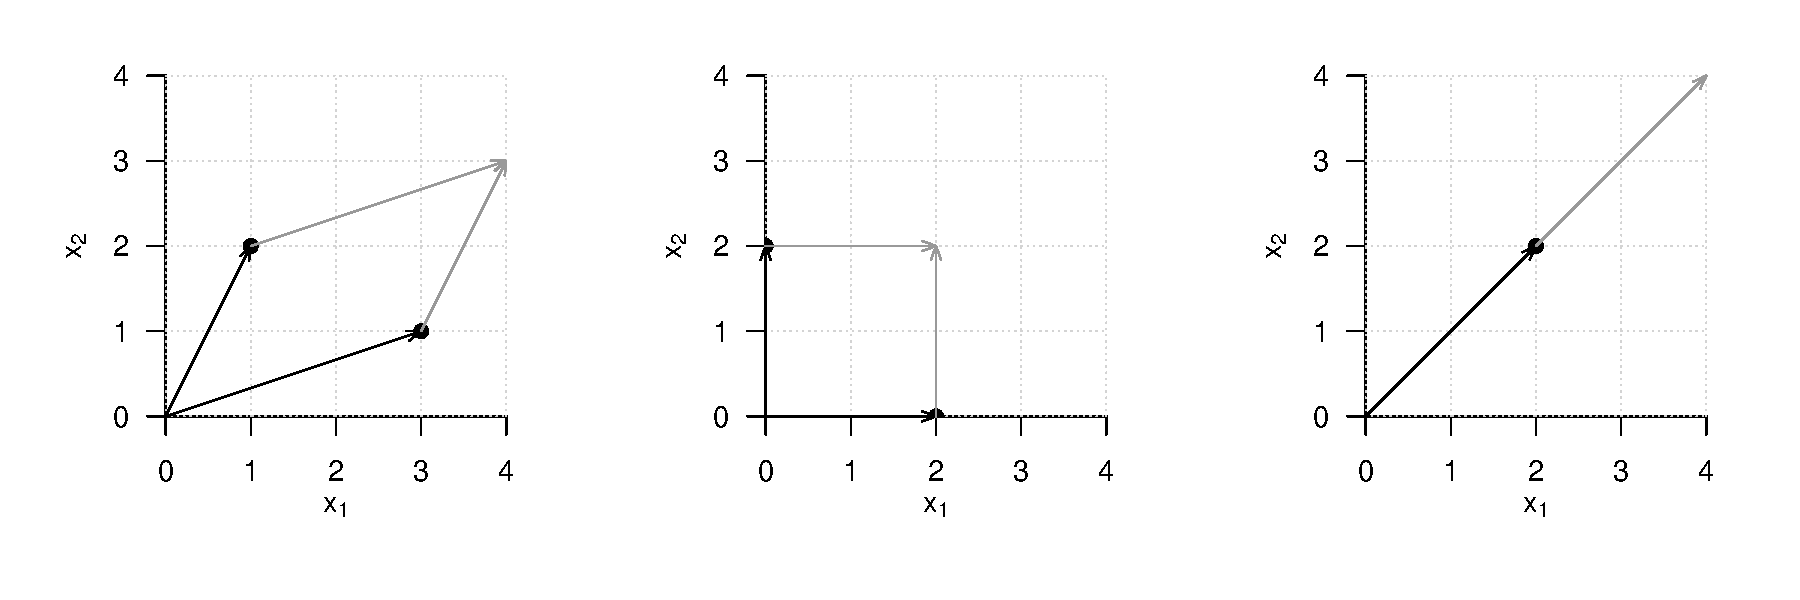
\includegraphics[width=1\linewidth]{3_Abbildungen/mvda_3_determinante} \end{center}
\vspace{-5mm}

\begin{equation*}
\det(A_1) =
3\cdot 2 - 1 \cdot 1 = 5
\quad\quad\quad\quad
\det(A_2) =
2\cdot 2 - 0 \cdot 0 = 4
\quad\quad\quad\quad
\det(A_3) =
2\cdot 2 - 2 \cdot 2 = 0
\end{equation*}
\end{frame}

\begin{frame}{}
\protect\hypertarget{section-6}{}
\large
\setstretch{2}
\vfill

Definition

Operationen

Determinanten

\textbf{Rang}

Spezielle Matrizen

Selbstkontrollfragen \vfill
\end{frame}

\begin{frame}{Rang}
\protect\hypertarget{rang}{}
\small

Überblick

\footnotesize
\setstretch{3}

\begin{itemize}
\tightlist
\item
  Der Rang einer Matrix ist eine Zahl an der bestimmte Eigenschaften der
  Matrix abgelesen werden können.
\item
  In dieser Hinsicht ist der Rang einer Matrix sehr ähnlich zur
  Determinante einer Matrix.
\item
  Viele Resultate in der linearen Algebra beruhen auf Annahmen über den
  Rang einer Matrix.
\item
  Der Rang einer Matrix ist ein tiefgehendes Konzept, das wir hier nur
  oberflächlich behandeln können.
\item
  Für ausführlichere Einführungen, siehe z.B. Searle (1982), Chapter 6
  und Strang (2009), Kapitel Chapter 3.2.
\item
  Wir verwenden hier einen Zugang über das Konzept der linearen
  Unabhängigkeit von Vektoren.
\item
  Wir erinnern zunächst an dieses Konzept.
\end{itemize}
\end{frame}

\begin{frame}{Rang}
\protect\hypertarget{rang-1}{}
\small
\begin{definition}[Rang einer Matrix]
\justifying
Es sei $A \in \mathbb{R}^{n \times m}$ und
\begin{equation}
a_1 :=
\begin{pmatrix}
a_{11} \\
\vdots \\
a_{n1}
\end{pmatrix},
a_2 :=
\begin{pmatrix}
a_{12} \\
\vdots \\
a_{n2}
\end{pmatrix},
...,
a_n :=
\begin{pmatrix}
a_{1m} \\
\vdots \\
a_{nm}
\end{pmatrix}
\in
\mathbb{R}^{n}
\end{equation}
seien die \textit{Spalten(vektoren)} von $A$. Dann ist \textit{der Rang von $A$}, 
geschrieben als $\mbox{rg}(A)$ definiert als die maximale Anzahl der linear unabhängigen
Spalten(vektoren) von $A$. Ist die Anzahl der maximal linear unabhängigen Spalten(vektoren)
von $A$ gleich $m$, so sagt man, dass \textit{$A$ vollen Spaltenrang hat}.
\end{definition}

\footnotesize

Bemerkungen

\begin{itemize}
\tightlist
\item
  Die Spalten einer Matrix werden hier als Vektoren in \(\mathbb{R}^n\)
  verstanden.
\item
  Die Definition macht keine Aussage darüber, wie der Rang einer Matrix
  zu bestimmen ist.
\item
  Es gibt verschiedene Algorithmen um den Rang einer Matrix zu
  bestimmen, wir vertiefen dies nicht.
\end{itemize}
\end{frame}

\begin{frame}{Rang}
\protect\hypertarget{rang-2}{}
Beispiele

\footnotesize

\noindent (1) Es sei \begin{equation}
X := \begin{pmatrix} 1 & 0  \\ 0 & 1  \\ 0 &  1  \end{pmatrix}
\end{equation} Dann ist sind die Spaltenvektoren keine skalaren
Vielfachen voneinander und damit linear unabhängig. Es gilt also
\(\mbox{rg}(X) = 2\).

\noindent (2) Es sei \begin{equation}
X := \begin{pmatrix} 1 & 2  \\ 1 & 2  \\ 0 &  0  \end{pmatrix}
\end{equation} Dann ist sind die Spaltenvektoren skalare Vielfache
voneinander. Die maximale Möglichkeit aus den Spaltenvektoren linear
unabhängige Vektoren auszuwählen ist also 1. Die maximale Anzahl an
linear unabhängigen Vektoren der Matrix ist als 1 und es gilt
\(\mbox{rg}(X) = 1\).

Bemerkungen

\begin{itemize}
\tightlist
\item
  In Beispiel (2) gerät die Definition des Rangs einer Matrix wie hier
  gegeben an ihre Grenze.
\item
  Alternative Definitionen, z.B. über die Dimension des Spaltenraumes
  sind eindeutiger, aber tiefgehender.
\item
  Die einzige Matrix mit Rang 0 ist die Nullmatrix.
\end{itemize}
\end{frame}

\begin{frame}[fragile]{Range}
\protect\hypertarget{range}{}
\vspace{1mm}

Beispiele

\footnotesize

\begin{Shaded}
\begin{Highlighting}[]
\CommentTok{\# Bestimmung des Matrixrangs in R über QR Zerlegung (https://de.wikipedia.org/wiki/QR{-}Zerlegung)}
\CommentTok{\# Beispiel (1)}
\NormalTok{X  }\OtherTok{=} \FunctionTok{matrix}\NormalTok{(}\FunctionTok{c}\NormalTok{(}\DecValTok{1}\NormalTok{,}\DecValTok{0}\NormalTok{,                          }\CommentTok{\# Matrixdefinition}
              \DecValTok{0}\NormalTok{,}\DecValTok{1}\NormalTok{,}
              \DecValTok{0}\NormalTok{,}\DecValTok{0}\NormalTok{),}
            \AttributeTok{nrow =} \DecValTok{3}\NormalTok{,}
            \AttributeTok{byrow =} \ConstantTok{TRUE}\NormalTok{)}
\NormalTok{rg }\OtherTok{=} \FunctionTok{qr}\NormalTok{(X)}\SpecialCharTok{$}\NormalTok{rank                             }\CommentTok{\# Rangevaluation}
\FunctionTok{print}\NormalTok{(rg)                                   }\CommentTok{\# Ausgabe}
\end{Highlighting}
\end{Shaded}

\begin{verbatim}
> [1] 2
\end{verbatim}

\begin{Shaded}
\begin{Highlighting}[]
\CommentTok{\# Beispiel (2)}
\NormalTok{X  }\OtherTok{=} \FunctionTok{matrix}\NormalTok{(}\FunctionTok{c}\NormalTok{(}\DecValTok{1}\NormalTok{,}\DecValTok{2}\NormalTok{,                          }\CommentTok{\# Matrixdefinition}
              \DecValTok{1}\NormalTok{,}\DecValTok{2}\NormalTok{,}
              \DecValTok{0}\NormalTok{,}\DecValTok{0}\NormalTok{),}
            \AttributeTok{nrow =} \DecValTok{3}\NormalTok{,}
            \AttributeTok{byrow =} \ConstantTok{TRUE}\NormalTok{)}
\NormalTok{rg }\OtherTok{=} \FunctionTok{qr}\NormalTok{(X)}\SpecialCharTok{$}\NormalTok{rank                             }\CommentTok{\# Rangevaluation}
\FunctionTok{print}\NormalTok{(rg)                                   }\CommentTok{\# Ausgabe}
\end{Highlighting}
\end{Shaded}

\begin{verbatim}
> [1] 1
\end{verbatim}
\end{frame}

\begin{frame}{Rang}
\protect\hypertarget{rang-3}{}
\small
\begin{theorem}[Rang und Invertierbarkeit]
\justifying
\normalfont
$A \in \mathbb{R}^{n \times n}$ sei eine Matrix. Dann gelten

\begin{itemize}
\item[(1)] $\mbox{rg}(A) = n \Leftrightarrow$ $A$ ist invertierbar.
\item[(2)] $\mbox{rg}(A) < n \Leftrightarrow$ $A$ ist nicht invertierbar.
\end{itemize}
\end{theorem}

\footnotesize

Bemerkung

\begin{itemize}
\tightlist
\item
  Wir verzichten auf einen Beweis.
\end{itemize}
\end{frame}

\begin{frame}{}
\protect\hypertarget{section-7}{}
\large
\setstretch{2}
\vfill

Definition

Operationen

Determinanten

Rang

\textbf{Spezielle Matrizen}

Selbstkontrollfragen \vfill
\end{frame}

\begin{frame}{Spezielle Matrizen}
\protect\hypertarget{spezielle-matrizen}{}
\footnotesize
\begin{definition}[Nullmatrizen, Einheitsmatrizen, Einheitsvektoren, Einsvektoren]
\begin{itemize}
\item Wir bezeichnen \textit{Nullmatrizen} mit
\begin{equation}
0_{nm} := (0)_{1 \le i \le n, 1 \le j \le m} \in \mathbb{R}^{n \times m}
\mbox{ und }
0_{n} := (0)_{1 \le i \le n} \in \mathbb{R}^{n}
\end{equation}
\item Wir bezeichnen die \textit{Einheitsmatrix} mit
\begin{equation}
I_{n} := (i_{jk})_{1 \le i \le n, 1 \le j \le n} \in \mathbb{R}^{n \times n} \mbox{ mit } i_{jk} = 1 \mbox{ für } j = k \mbox{ und } i_{jk} = 0 \mbox{ für } j \neq k
\end{equation}
\item Wir bezeichnen die \textit{Einheitsvektoren} $e_i, i = 1,...,n$ mit
\begin{equation}
e_{i} := (e_{{i}_j})_{1 \le j \le n} \in \mathbb{R}^{n} \mbox{ mit } e_{{i}_j} = 1 \mbox{ für } i = j \mbox{ und } e_{{i}_j} = 0 \mbox{ für } i \neq j
\end{equation}
\item Wir bezeichnen den \textit{Einsvektor} mit
\begin{equation}
1_n := (1)_{1 \le i \le n} \in \mathbb{R}^n
\end{equation}
\end{itemize}
\end{definition}

Bemerkungen

\begin{itemize}
\tightlist
\item
  \(0_{nm}\) und \(0_{n}\) bestehen nur aus Nullen.
\item
  \(I_{n}\) besteht nur aus Nullen und Diagonalelementen gleich Eins.
\item
  \(e_i, i 1,....,n\) besteht nur aus Nullen und einer Eins in der
  \(i\)ten Komponente.
\item
  \(1_n\) besteht nur aus Einsen.
\end{itemize}
\end{frame}

\begin{frame}{Spezielle Matrizen}
\protect\hypertarget{spezielle-matrizen-1}{}
\footnotesize
\begin{definition}[Symmetrische, diagonale, und orthogonale Matrizen]
\begin{itemize}
\item Eine Matrix $S \in \mathbb{R}^{n \times n}$ heißt \textit{symmetrisch}, wenn gilt dass $S^T = S$.
\item Eine Matrix $D \in \mathbb{R}^{n \times n}$ heißt \textit{Diagonalmatrix}, wenn $d_{ij} = 0$ für $1 \le i,j \le n, i \neq j$.
\item Eine Matrix $Q \in \mathbb{R}^{n \times n}$ heißt \textit{orthogonal}, wenn ihre Spaltenvektoren wechselseitig \textit{orthonormal} sind.
\end{itemize}
\end{definition}

Bemerkungen

\begin{itemize}
\justifying
\item Eine Diagonalmatrix $D$ mit Diagonalelementen $d_1,...,d_n$ schreibt man auch als $ D= \mbox{diag}(d_1,...,d_n)$.
\item Symmetrische, diagonale, und orthogonale Matrizen haben viele ``gute'' Eigenschaften.
\item Zum Beispiel überzeugt man sich einfach davon, dass Multiplikation einer Matrix $A$ 
von links mit einer Diagonalmatrix $D$ der Multiplikation der Zeilen der Matrix $A$ 
mit den entsprechenden Diagonaleinträgen von $D$ entspricht. Die entsprechende 
Multiplikation von rechts entspricht der Multiplikation der Spalten von $A$ mit 
entsprechenden Diagonaleinträgen von $D$.
\item Eine weitere im Folgenden wichtige Eigenschaft von Diagonalmatrizen ist
\begin{itemize}
\begin{footnotesize}
\item[$\circ$] $D := \mbox{diag}(d_1,...,d_n)$ ist eine Diagonalmatrix $\Rightarrow$ $\det(D) = \prod_{i=1}^n d_i$.
\end{footnotesize}
\end{itemize}
\end{itemize}
\end{frame}

\begin{frame}{Spezielle Matrizen}
\protect\hypertarget{spezielle-matrizen-2}{}
\small
\begin{definition}[Positiv-definite Matrix]
Eine quadratische Matrix $C \in \mathbb{R}^{n \times n}$ heißt positiv-definit ($\mbox{p.d.}$), wenn
\begin{itemize}
\item $C$ eine symmetrische Matrix ist und
\item für alle $x \in \mathbb{R}^n, x \neq 0_n$ gilt, dass $x^TCx > 0$ ist.
\end{itemize}
\end{definition}

\footnotesize

Bemerkungen

\begin{itemize}
\tightlist
\item
  Im LGM Kontext sind \(\mbox{p.d.}\) Matrizen für die Definition der
  multivariaten Normalverteilungen grundlegend.
\item
  Wir werden einige Aussagen zu positiv-definiten Matrizen für die LGM
  Theorie benötigen.
\item
  Wir halten dieses Aussagen hier ohne Beweis fest und verweisen für
  Beweise auf die einschlägige Literatur
\end{itemize}

\begin{enumerate}
[(1)]
\tightlist
\item
  Jede positiv-definite Matrix ist invertierbar.
\item
  Die Inverse einer positiv-definiten Matrix ist ebenfalls
  positiv-definit.
\end{enumerate}
\end{frame}

\begin{frame}{}
\protect\hypertarget{section-8}{}
\large
\setstretch{2}
\vfill

Definition

Operationen

Determinanten

Rang

Spezielle Matrizen

\textbf{Selbstkontrollfragen}

\vfill
\end{frame}

\begin{frame}{Selbstkontrollfragen}
\protect\hypertarget{selbstkontrollfragen}{}
\footnotesize
\begin{enumerate}
\item Geben Sie die Definition einer Matrix wieder.
\item Nennen Sie sechs Matrixoperationen.
\item Geben Sie die Definitionen der Matrixaddition und -subtraktion wieder.
\item Geben Sie die Definition der Skalarmultiplikation für Matrizen wieder.
\item Geben Sie die Definition der Matrixtransposition wieder.
\item Es seien
\begin{equation}
A :=
\begin{pmatrix*}[r]
1 & 2 \\
2 & 1
\end{pmatrix*},
B :=
\begin{pmatrix*}[r]
3 & 0 \\
1 & 2
\end{pmatrix*},
\mbox{ und }
c := 2
\end{equation}
Berechnen Sie
\begin{equation}
D := c\left(A - B^T\right)
\mbox{ und }
E := \left(cA\right)^T + B.
\end{equation}
per Hand und überprüfen Sie Ihre Rechnung mit R.


\item Geben Sie die Definition der Matrixmultiplikation wieder.
\item Es seien $A \in \mathbb{R}^{3 \times 2}, B \in \mathbb{R}^{2\times 4}$
und $C \in \mathbb{R}^{3 \times 4}$. Prüfen Sie, ob folgende Matrixprodukte
definiert sind, und wenn ja, geben Sie die Größe der resultierenden Matrix an:
\begin{equation}
ABC, \quad ABC^T, \quad, A^TCB^T \quad, BAC.
\end{equation}

\end{enumerate}
\end{frame}

\begin{frame}{Selbstkontrollfragen}
\protect\hypertarget{selbstkontrollfragen-1}{}
\footnotesize
\begin{enumerate}
\setcounter{enumi}{8}
\item Es seien
\begin{equation}
A :=
\begin{pmatrix*}[r]
1 & 2 & 3 \\
4 & 5 & 6 \\
3 & 2 & 0
\end{pmatrix*}
B :=
\begin{pmatrix*}[r]
1 & 2 & 2 \\
1 & 3 & 1 \\
2 & 0 & 0
\end{pmatrix*}
\mbox{ und }
C :=
\begin{pmatrix*}[r]
1 \\ 3 \\ 2
\end{pmatrix*}.
\end{equation}
Berechnen Sie die Matrixprodukte
\begin{equation}
AB , \quad\quad
B^TA^T, \quad\quad
\left(B^TA^T\right)^T, \quad\quad
AC
\end{equation}
per Hand und überprüfen Sie Ihre Rechnung mit R.



\item Invertieren Sie die Matrizen $A$ und $B$ aus der vorherigen Aufgabe mithilfe
von solve() oder matlib::inv()  und überprüfen Sie die Inverseeigenschaft der 
inversen Matrizen mithilfe von R.



\item Geben Sie die Formel für die Determinante von $A := (A_{ij})_{1 \le i,j \le 2} \in \mathbb{R}^2$ wieder.
\item Geben Sie die Formel für die Determinante von $A := (A_{ij})_{1 \le i,j \le 3} \in \mathbb{R}^3$ wieder.
\item Berechnen Sie die Determinanten von
\begin{equation}
A := \begin{pmatrix} 2 & 1 \\ 1 & 2 \end{pmatrix}
B := \begin{pmatrix} 3 & 2 & 1 \\ 2 & 3 & 2 \\ 1 & 2 & 3 \end{pmatrix} \mbox{ und }
C := \mbox{diag}(1,2,3)
\end{equation}
per Hand und überprüfen Sie Ihre Rechnung mit R.
\end{enumerate}
\end{frame}

\begin{frame}{Selbstkontrollfragen}
\protect\hypertarget{selbstkontrollfragen-2}{}
\footnotesize
\setstretch{1.6}
\begin{enumerate}
\setcounter{enumi}{13}
\item Geben Sie den Determinantenmultiplikationssatz wieder.
\item Geben Sie das Theorem zur Invertierbarkeit und Determinante von Matrizen wieder.
\item Geben Sie die Definition des Rangs einer Matrix wieder.
\item Wann sagt man, dass eine Matrix vollen Spaltenrang hat?
\item Bestimmen Sie dien Rang folgender Matrizen durch überlegen und mithilfe von R
\begin{equation}
X_1 = \begin{pmatrix} 1 & 1 \\ 1 & 2 \\ 1 & 3\end{pmatrix},
X_2 = \begin{pmatrix} 1 & 1 & 0\\ 1 & 1 & 0 \\ 1 & 0 & 1 \\ 1 & 0 & 1\end{pmatrix},
X_3 = \begin{pmatrix} 1 & 0\\ 1 & 0 \\ 1 & 1 \\ 1 & 1\end{pmatrix}.
\end{equation}
\item Geben Sie die Definition einer symmetrischen Matrix wieder.
\item Geben Sie die Definition einer Diagonalmatrix wieder.
\item Geben Sie die Definition einer orthogonalen Matrix wieder.
\item Geben Sie die Definition einer positiv-definiten Matrix wieder.
\end{enumerate}
\end{frame}

\begin{frame}{References}
\protect\hypertarget{references}{}
\footnotesize

\hypertarget{refs}{}
\begin{CSLReferences}{1}{0}
\leavevmode\vadjust pre{\hypertarget{ref-searle_1982}{}}%
Searle, Shayle. 1982. \emph{Matrix {Algebra Useful} for {Statistics}}.
{Wiley-Interscience}.

\leavevmode\vadjust pre{\hypertarget{ref-strang_2009}{}}%
Strang, Gilbert. 2009. \emph{Introduction to {Linear Algebra}}.

\end{CSLReferences}
\end{frame}

\end{document}
